% rubber: setlist arguments --shell-escape

\newif\iffinal\finaltrue
\newif\ifnotes\notestrue
% draft hides fancy stuff

\pdfminorversion=4

\documentclass[compress,t,usenames,dvipsnames]{beamer}
\usetheme{Custom}

\usepackage{keycommand}
\usepackage[T1]{fontenc}
\usepackage[utf8]{inputenc}
\usepackage[english]{babel}
\usepackage{floatflt}
\usepackage{colortbl}
\usepackage{graphicx}
\usepackage{tikz}
\usepackage{pgfplots}
\usepackage{listings}
\usepackage{multicol}
\usepackage{multirow}
\usepackage{array}
\usepackage{eurosym}
\usepackage{minted}
\usepackage{hyperref}
\usepackage{caption}
\usepackage{siunitx}
\usepackage{adjustbox}

\usepackage[backend=biber,style=numeric,natbib=true]{biblatex}
\addbibresource{../common/sources.bib}

\usetikzlibrary{shapes,arrows,calc,decorations.markings,automata,matrix,intersections}

% http://www.logicmatters.net/resources/pdfs/MathFonts.pdf
\usepackage{kerkis} % Kerkis roman and sans
\usepackage{kmath}

\usepackage{pgfpages}

\newcommand{\tabitem}{~~\llap{\textbullet}~~}
\ifnotes
    \setbeamertemplate{note page}[plain]
    \setbeameroption{show notes on second screen=right}
    \AtBeginNote{\hspace*{-20pt}\addtolength\leftmargini{-20pt}}
    \AtEndNote{\addtolength\leftmargini{20pt}}
\fi

\title{Prototype for a virtual keyboard based on IMUs and machine learning}
\author{Paul Bienkowski \& Carolin Konietzny}
\institute{TAMS, Fachbereich Informatik, Universität Hamburg}
\date{2017-05-16}
\setbeamerfont{note page}{size=\small}

%%%%%%%%%%%%%%%%%%%%%%%%%%%%%%%%%%%%%%%%%%%%%%%%%%%%%%%%%%%%%%%%%%%%5
%%% Packages

\usepackage{geometry}
\usepackage[utf8]{inputenc}
\usepackage[T1]{fontenc}
\usepackage[pdftex]{graphicx}
\usepackage[ngerman]{babel}
\usepackage{colortbl}
\usepackage{soul}
\usepackage{textcomp}
\usepackage[usenames,dvipsnames]{xcolor}
\usepackage[toc,page]{appendix}
\usepackage{amssymb}
\usepackage{amsmath}
\usepackage{enumerate}
\usepackage{tikz}
\usepackage[hidelinks]{hyperref}
\usepackage{lastpage}
\usepackage{nameref}
\usepackage{etoolbox}
\usepackage[binary-units=true]{siunitx}
\usepackage{eurosym}
\usepackage{wrapfig}
\usepackage{multirow,bigdelim}
\usepackage{multicol}
\usepackage{pgfplots}
\usepackage{listings}
\usepackage{array}
\usepackage[within=none]{caption}
\usepackage{adjustbox}
\usepackage{xspace}
\usepackage[inline]{enumitem}
\usepackage{booktabs}
\usepackage{tabularx}
\usepackage{subcaption}
% \usepackage{float}
\usepackage{titlesec}
\usepackage[backend=biber,labelnumber,defernumbers=true,style=authoryear,natbib=true]{biblatex}
\usepackage{makecell}
\usepackage{minted}
\usepackage{nicefrac}
\usepackage{csquotes}
\usepackage{lipsum}
\usepackage{rotating}
\usepackage{pdflscape}
\usepackage{afterpage}
\usepackage{ltablex}
\usepackage{keycommand}

\let\tmp\oddsidemargin
\let\oddsidemargin\evensidemargin
\let\evensidemargin\tmp
\reversemarginpar

% rubber: setlist arguments --shell-escape
%%%%%%%%%%%%%%%%%%%%%%%%%%%%%%%%%%%%%%%%%%%%%%%%%%%%%%%%%%%%%%%%%%%%5
%%% Helper macros for different types of TODOs

\newcommand{\factcheck}{\textcolor{orange}{\textsuperscript{\textbf{!!}}}~}
\newcommand{\citationneeded}{\textcolor{blue}{\textsuperscript{\textbf{??}}}~}
\newcommand{\cn}{\citationneeded} % alias for \citationneeded
\newcommand{\todo}{\textcolor{green}{TODO!}}

%%%%%%%%%%%%%%%%%%%%%%%%%%%%%%%%%%%%%%%%%%%%%%%%%%%%%%%%%%%%%%%%%%%%5
%%% References

\newcommand{\figlabel}[1]{\label{fig:#1}}
\newcommand{\chaplabel}[1]{\label{chap:#1}}
\newcommand{\seclabel}[1]{\label{sec:#1}}
\newcommand{\tablabel}[1]{\label{tab:#1}}
\newcommand{\subseclabel}[1]{\label{subsec:#1}}
\newcommand{\lstlabel}[1]{\label{lst:#1}}

\newcommand{\figref}[1]{\figurename~\ref{fig:#1}}
\newcommand{\chapref}[1]{\chaptername~\ref{chap:#1}}
\newcommand{\secref}[1]{\secname~\ref{sec:#1}}
\newcommand{\tabref}[1]{\tablename~\ref{tab:#1}}
\newcommand{\subsecref}[1]{\subsecname~\ref{subsec:#1}}
\newcommand{\lstref}[1]{\listingscaption~\ref{lst:#1}}

\newcommand{\Figref}[1]{\figref{#1} ,,\nameref{fig:#1}''}
\newcommand{\Chapref}[1]{\chapref{#1} ,,\nameref{chap:#1}''}
\newcommand{\Secref}[1]{\secref{#1} ,,\nameref{sec:#1}''}
\newcommand{\Tabref}[1]{\tabref{#1} ,,\nameref{tab:#1}''}
\newcommand{\Subsecref}[1]{\subsecref{#1} ,,\nameref{subsec:#1}''}
\newcommand{\Lstref}[1]{\lstref{#1} ,,\nameref{lst:#1}''}

% use for referencing a chapter inside a \cite, e.g. \cite[\citechap{5}]{mycite}
\newcommand{\citechap}[1]{Kapitel~#1}

% Optinally rename headings :)
%\addto\captionsngerman{\renewcommand{\chaptername}{Kap.}}
%\addto\captionsngerman{\renewcommand{\figurename}{Abb.}}
%\addto\captionsngerman{\renewcommand{\tablename}{Tab.}}
%\addto\captionsngerman{\renewcommand{\sectionname}{Abschn.}}
%\addto\captionsngerman{\renewcommand{\subsectionname}{U.-abschn.}}
\renewcommand{\listingscaption}{Codebeispiel}
\newcommand{\secname}{Abschnitt}
\newcommand{\subsecname}{Unterabschnitt}


%%%%%%%%%%%%%%%%%%%%%%%%%%%%%%%%%%%%%%%%%%%%%%%%%%%%%%%%%%%%%%%%%%%%5
%%% Tikz style rules and configuration

\usetikzlibrary{calc}
\usetikzlibrary{fit}
\usetikzlibrary{shapes}
\usetikzlibrary{arrows}
\usetikzlibrary{shapes.misc}
\usetikzlibrary{positioning}
\usetikzlibrary{shapes.geometric}
\usetikzlibrary{decorations.markings}
\usetikzlibrary{decorations.pathreplacing}
\usetikzlibrary{shadows}
\usetikzlibrary{automata}
\usetikzlibrary{matrix}
\usetikzlibrary{intersections}
\tikzset{
    keyboardkey/.style={
      draw,
      fill=white,
      drop shadow={shadow xshift=0.25ex,shadow yshift=-0.25ex,fill=black,opacity=0.75},
      rectangle,
      rounded corners=1pt,
      inner sep=2pt,
      minimum height=12pt,
      minimum width=1em,
      line width=0.5pt,
      font=\scriptsize\sffamily
    },
    onslide/.code args={<#1>#2}{% http://tex.stackexchange.com/a/6155/16595
        \only<#1>{\pgfkeysalso{#2}}
    },
    flowchart node/.style={
        rectangle,
        rounded corners,
        minimum width=3cm,
        minimum height=0.8cm,
        text width=3cm,
        align=center,
        draw=black,
        fill=white,
        thick,
        font=\scriptsize,
    },
    flowchart arrow/.style={
        thick,
        ->,
        >=stealth,
    },
}
\pgfplotsset{
    /pgfplots/xlabel near ticks/.style={
        /pgfplots/every axis x label/.style={
            at={(ticklabel cs:0.5)},
            anchor=near ticklabel
        }
    },
    /pgfplots/ylabel near ticks/.style={
        /pgfplots/every axis y label/.style={
            at={(ticklabel cs:0.5)},
            rotate=90,
            anchor=near ticklabel
        }
    }
}

%%%%%%%%%%%%%%%%%%%%%%%%%%%%%%%%%%%%%%%%%%%%%%%%%%%%%%%%%%%%%%%%%%%%5
%%% Text formatting commands

\newcommand{\imagesource}[1]{\par\vspace{2mm}\tiny{}Bildquelle: \url{#1}}
\newcommand{\productname}[1]{\textsc{#1}}
\newcommand{\fremdwort}[1]{\emph{#1}}
\DeclareRobustCommand\keyboard[1]{%
    \tikz[baseline={($(key) + (0, -3pt)$)}]\node[keyboardkey] (key) {\textbf{#1}};
}
\newcommand{\shift}{$\Uparrow$}
\newcommand{\return}{\rotatebox[origin=c]{180}{$\Rsh$}}
\newcommand{\spacebar}{\textvisiblespace{}}

\newcommand{\iic}{I\textsuperscript{2}C\xspace}

%%%%%%%%%%%%%%%%%%%%%%%%%%%%%%%%%%%%%%%%%%%%%%%%%%%%%%%%%%%%%%%%%%%%5
%%% Title formats

\titleformat{\chapter}{\normalfont\huge\bfseries}{\thechapter}{2em}{}
\titleformat{\section}{\normalfont\Large\bfseries}{\thesection}{1em}{}
\titleformat{\subsection}{\normalfont\large\bfseries}{\thesubsection}{1em}{}
\titleformat{\subsubsection}{\normalfont\bfseries}{\thesubsubsection}{1em}{}

%%%%%%%%%%%%%%%%%%%%%%%%%%%%%%%%%%%%%%%%%%%%%%%%%%%%%%%%%%%%%%%%%%%%5
%%% Spacing

\setlength{\parindent}{0pt}
\setlength{\parskip}{1.5ex}
\newcommand{\only}[1]{}

%%%%%%%%%%%%%%%%%%%%%%%%%%%%%%%%%%%%%%%%%%%%%%%%%%%%%%%%%%%%%%%%%%%%5
%%% Layouting rules

% Don't spread text vertically on the page
\raggedbottom
% Try not to split footnotes
\interfootnotelinepenalty=10000
% \floatplacement{figure}{tb}

%%%%%%%%%%%%%%%%%%%%%%%%%%%%%%%%%%%%%%%%%%%%%%%%%%%%%%%%%%%%%%%%%%%%5
%%% Itemization style

\renewcommand{\labelitemi}{--}
\renewcommand{\labelitemii}{$\rightarrow$}
\renewcommand{\labelitemiii}{$\bullet$}
\renewcommand{\labelitemiv}{$\bullet$}

% \renewcommand{\labelenumi}{\theenumi.}
% \renewcommand{\labelenumii}{(\theenumii)}
% \renewcommand{\labelenumiii}{\theenumiii.}
% \renewcommand{\labelenumiv}{\theenumiv}

%%%%%%%%%%%%%%%%%%%%%%%%%%%%%%%%%%%%%%%%%%%%%%%%%%%%%%%%%%%%%%%%%%%%5
%%% Font family

% \renewcommand{\familydefault}{\sfdefault}
\sisetup{math-rm=\mathsf,text-rm=\sffamily,per-mode=symbol}

%%%%%%%%%%%%%%%%%%%%%%%%%%%%%%%%%%%%%%%%%%%%%%%%%%%%%%%%%%%%%%%%%%%%5
%%% Color defintiions

\definecolor{uhhred}{RGB}{226,0,26}
\definecolor{primary}{RGB}{226,0,26}
\definecolor{secondary}{RGB}{78,78,78}

% Some plot colors, same scheme that matplotlib uses by default
\definecolor{plot0}{HTML}{0072bd}
\definecolor{plot1}{HTML}{d95319}
\definecolor{plot2}{HTML}{edb120}
\definecolor{plot3}{HTML}{7e2f8e}
\definecolor{plot4}{HTML}{77ac30}
\definecolor{plot5}{HTML}{4dbeee}
\definecolor{plot6}{HTML}{a2142f}


%%%%%%%%%%%%%%%%%%%%%%%%%%%%%%%%%%%%%%%%%%%%%%%%%%%%%%%%%%%%%%%%%%%%5
%%% Bibliography
\addbibresource{../common/sources.bib}

\DeclareFieldFormat{labelnumberwidth}{\mkbibbrackets{#1}}

% \usepackage{xpatch}
% \xpretobibmacro{author}{\mkbibbold\bgroup}{}{}
% \xapptobibmacro{author}{\egroup}{}{}
% \xpretobibmacro{bbx:editor}{\mkbibbold\bgroup}{}{}
% \xapptobibmacro{bbx:editor}{\egroup}{}{}
% \renewcommand*{\labelnamepunct}{\mkbibbold{\addcolon\space}}
\setlength{\bibitemsep}{1ex}
% \setlength{\bibhang}{3ex}

\newcommand{\letbibmacro}[2]{%
  \csletcs{abx@macro@#1}{abx@macro@#2}%
}
\letbibmacro{original-cite}{cite}

\renewbibmacro*{cite}{%
  \printtext[bibhyperref]{%
    \printfield{labelprefix}%
    \ifentrytype{online}
      {\printfield[labelnumberwidth]{labelnumber}}
      {\usebibmacro{original-cite}}}}

\defbibenvironment{bibliographyNUM}
  {\list
     {\printtext[labelnumberwidth]{%
        \printfield{prefixnumber}%
        \printfield{labelnumber}}}
     {\setlength{\labelwidth}{\labelnumberwidth}%
      \setlength{\leftmargin}{\labelwidth}%
      \setlength{\labelsep}{\biblabelsep}%
      \addtolength{\leftmargin}{\labelsep}%
      \setlength{\itemsep}{\bibitemsep}%
      \setlength{\parsep}{\bibparsep}}%
      \renewcommand*{\makelabel}[1]{\hss##1}}
  {\endlist}
  {\item}

\assignrefcontextkeyws[sorting=none]{online}

%%%%%%%%%%%%%%%%%%%%%%%%%%%%%%%%%%%%%%%%%%%%%%%%%%%%%%%%%%%%%%%%%%%%5
%%% Code listings
\usepackage[scaled]{beramono}
\setminted{
    framerule=1pt,
    xleftmargin=5mm,
    baselinestretch=1.0,
    style=colorful,
    linenos,
    fontsize=\small,
}
\let\oldinputminted\inputminted
\usepackage{mdframed}
\renewcommand{\inputminted}[2]{%
    \begin{mdframed}%
        \oldinputminted{#1}{#2}%
    \end{mdframed}%
}

\newkeycommand\drawkeyboard[scale=1,4=white,5=white,6=white,7=white,8=white,9=white,0=white,minus=white,equalsign=white,backspace=white,r=white,t=white,y=white,u=white,i=white,o=white,p=white,lbracket=white,rbracket=white,backslash=white,f=white,g=white,h=white,j=white,k=white,l=white,semi=white,tick=white,return=white,c=white,v=white,b=white,n=white,m=white,comma=white,dot=white,slash=white,shift=white,space=white,alt=white,meta=white,menu=white,ctrl=white]{%
    \scalebox{\commandkey{scale}}{
        \sffamily
        \begin{tikzpicture}[
            remember picture,
            keyboard key/.code args={##1}{
                \pgfkeysalso{
                    draw,
                    rectangle,
                    minimum width=6mm,
                    minimum height=6mm,
                    inner sep=0pt,
                    font=\small,
                    fill={\commandkey{##1}}
                }
            },
            legend/.style={
                draw,
                rectangle,
                minimum width=3mm,
                minimum height=3mm,
            },
        ]
            \node[keyboard key=g] (g) at (0, 0) {G};
            \node[keyboard key=h,right=1mm of g] (h) {H};
            \node[keyboard key=j,right=1mm of h] (j) {J};
            \node[keyboard key=k,right=1mm of j] (k) {K};
            \node[keyboard key=l,right=1mm of k] (l) {L};
            \node[keyboard key={semi},right=1mm of l] (semi) {;};
            \node[keyboard key={tick},right=1mm of semi] (tick) {\textquotesingle};
            \node[keyboard key={backslash},right=1mm of tick] (backslash) {\textbackslash};

            \node[keyboard key=b,below right=1mm and -4mm of g] (b) {B};
            \node[keyboard key=n,right=1mm of b] (n) {N};
            \node[keyboard key=m,right=1mm of n] (m) {M};
            \node[keyboard key={comma},right=1mm of m] (comma) {,};
            \node[keyboard key={dot},right=1mm of comma] (dot) {.};
            \node[keyboard key={slash},right=1mm of dot] (slash) {/};
            \node[keyboard key={shift},right=1mm of slash,minimum width=16mm] (shift) {$\uparrow$};

            \node[keyboard key=t,above left=1mm and -4mm of g] (t) {T};
            \node[keyboard key=y,right=1mm of t] (y) {Y};
            \node[keyboard key=u,right=1mm of y] (u) {U};
            \node[keyboard key=i,right=1mm of u] (i) {I};
            \node[keyboard key=o,right=1mm of i] (o) {O};
            \node[keyboard key=p,right=1mm of o] (p) {P};
            \node[keyboard key={lbracket},right=1mm of p] (lbracket) {[};
            \node[keyboard key={rbracket},right=1mm of lbracket] (rbracket) {]};

            \node[keyboard key=5,above left=1mm and -4mm of t] (5) {5};
            \node[keyboard key=6,right=1mm of 5] (6) {6};
            \node[keyboard key=7,right=1mm of 6] (7) {7};
            \node[keyboard key=8,right=1mm of 7] (8) {8};
            \node[keyboard key=9,right=1mm of 8] (9) {9};
            \node[keyboard key=0,right=1mm of 9] (0) {0};
            \node[keyboard key={minus},right=1mm of 0] (minus) {-};
            \node[keyboard key={equalsign},right=1mm of minus] (equalsign) {=};
            \node[keyboard key={backspace},right=1mm of equalsign,minimum width=8mm] (backspace) {$\leftarrow$};

            \node[keyboard key={space},below=1mm of b,minimum width=38mm] (space) {\textvisiblespace};
            \node[keyboard key={alt},font=\tiny,right=1mm of space,minimum width=7mm] (alt) {Alt};
            \node[keyboard key={meta},font=\tiny,right=1mm of alt,minimum width=7mm] (meta) {Meta};
            \node[keyboard key={menu},font=\tiny,right=1mm of meta,minimum width=7mm] (menu) {Menu};
            \node[keyboard key={ctrl},font=\tiny,right=1mm of menu,minimum width=11mm] (ctrl) {Ctrl};

            \node[keyboard key=v,left=1mm of b] (v) {V};
            \node[keyboard key=c,left=1mm of v] (c) {C};
            \node[keyboard key=f,left=1mm of g] (f) {F};
            \node[keyboard key=r,left=1mm of t] (r) {R};
            \node[keyboard key=4,left=1mm of 5] (4) {4};

            \path[keyboard key={return}]
                ($(backslash.north east) + (1mm, 1mm) $) --
                ++(0, -7mm) --
                ++(4mm, 0) --
                ++(0, 13mm) --
                ++(-6mm, 0) --
                ++(0, -6mm) --
                ($(backslash.north east) + (1mm, 1mm) $);
            \node[anchor=center] (return) at ($ (rbracket.center) + (7mm, 0) $)
            {\return};

            \node[legend,label=right:{\scriptsize{}Daumen},fill=thumb,right=3mm of backspace.south east,anchor=north west] (thumb) {};
            \node[legend,label=right:{\scriptsize{}Zeigefinger},fill=indexfinger,below=1mm of thumb] (index) {};
            \node[legend,label=right:{\scriptsize{}Mittelfinger},fill=middlefinger,below=1mm of index] (middle) {};
            \node[legend,label=right:{\scriptsize{}Ringfinger},fill=ringfinger,below=1mm of middle] (ring) {};
            \node[legend,label=right:{\scriptsize{}Kleiner Finger},fill=pinky,below=1mm of ring] (pinky) {};
        \end{tikzpicture}
    }
}

\definecolor{thumb}{HTML}{CE93D8}
\definecolor{indexfinger}{HTML}{90CAF9}
\definecolor{middlefinger}{HTML}{E6EE9C}
\definecolor{ringfinger}{HTML}{EF9A9A}
\definecolor{pinky}{HTML}{FFF59D}

\colorlet{thumb}{plot0}
\colorlet{indexfinger}{plot1}
\colorlet{middlefinger}{plot2}
\colorlet{ringfinger}{plot3}
\colorlet{pinky}{plot4}

\newcommand\phasekeyboardslide[1]{
    \begin{tikzpicture}[remember picture,overlay]
        \node[anchor=north east,fill=white!90!black,yshift=-16pt] at (current page.north east) {%
            \phasekeyboard{#1}
        };
    \end{tikzpicture}
}

\newcommand\phasekeyboard[1]{
    \IfEqCase{#1}{%
        {1}{\drawkeyboard[scale=0.8,n=indexfinger, h=indexfinger]{}}%
        {2}{\drawkeyboard[scale=0.8,space=thumb, y=indexfinger, b=indexfinger, g=indexfinger, t=indexfinger, n=indexfinger, h=indexfinger, u=middlefinger, j=middlefinger, m=middlefinger,]{}}%
        {3}{\drawkeyboard[scale=0.8,y=indexfinger,h=indexfinger,n=indexfinger,u=indexfinger,j=indexfinger,m=indexfinger,i=middlefinger,k=middlefinger,comma=middlefinger,
        o=ringfinger,l=ringfinger,dot=ringfinger,p=pinky,semi=pinky,slash=pinky,lbracket=pinky,rbracket=pinky,tick=pinky,backslash=pinky,space=thumb,return=pinky,shift=pinky]{}}%
    }[\PackageError{phasekeyboard}{Undefined option to phasekeyboard: #1}{}]
}


\begin{document}

\tikzset{
    onslide/.code args={<#1>#2}{% http://tex.stackexchange.com/a/6155/16595
        \only<#1>{\pgfkeysalso{#2}}
    },
    flowchart node/.style={
        rectangle,
        rounded corners,
        minimum width=3cm,
        minimum height=0.8cm,
        text width=3cm,
        align=center,
        draw=black,
        fill=white,
        thick,
        font=\scriptsize,
    },
    flowchart arrow/.style={
        thick,
        ->,
        >=stealth,
    },
}


\frontmatter{}
\frontmatter
\newgeometry{centering,left=2cm,right=2cm,top=2cm,bottom=2cm}
\begin{titlepage}
\includegraphics[scale=0.3]{UHH-Logo_2010_Farbe_CMYK.pdf}
\vspace*{2cm}
\Large
\begin{center}{\color{uhhred}\textbf{\so{BACHELORTHESIS}}}
\vspace*{2.0cm}\\
{\LARGE \textbf{Prototyp für eine virtuelle Tastatur basierend auf IMUs und maschinellem Lernen - Anwendung}}
\vspace*{2.0cm}\\
vorgelegt von
\vspace*{0.4cm}\\
Carolin Konietzny
\end{center}

\vspace*{3.9cm}

\noindent
MIN-Fakultät \vspace*{0.4cm} \\
Fachbereich Informatik \vspace*{0.4cm} \\
Arbeitsbereich Technische Aspekte Multimodaler Systeme \vspace*{0.4cm} \\
Studiengang: Informatik \vspace*{0.4cm} \\
Matrikelnummer: 6523939 \vspace*{0.8cm} \\
Erstgutachter: Dr.~Norman Hendrich \vspace*{0.4cm} \\
Zweitgutachter: Florens Wasserfall

\end{titlepage}

\restoregeometry{}

\cleardoublepage
\hspace{0pt}
\vfill
\begin{center}
\begin{minipage}{0.7\textwidth}
    \begin{center}
        \textsc{Kurzbeschreibung}
    \end{center}
    \vspace{-2ex}
    \noindent\rule[0.5ex]{\linewidth}{0.5pt}
    Das Projekt ,,Prototyp für eine virtuelle Tastatur basierend auf IMUs und maschinellem Lernen'' zielt darauf ab, ein System zu entwickeln, das als Alternative zu einer traditionellen Computertastatur Texteingaben aus den beim Tippen gemachten Bewegungen ermittelt. In dieser Arbeit wird ein Verfahren erläutert, aus den Bewegungsdaten von 6 IMUs, welche an den Fingern und der Rückseite einer Hand angebracht sind, die beim Tippen durchgeführten Tastenanschläge zu bestimmen. Hierzu werden die benötigten Vorverarbeitungsschritte vorgestellt und gezeigt, dass die ein \fremdwort{Convolutional Neural Network} für diese Aufgabe sehr geeignet ist. Bei langsamem Tippen von 10 verschiedenen Tasten konnte eine Genauigkeit von 85\% erreicht werden.
\end{minipage}
\\[2cm]
    \begin{minipage}{0.7\textwidth}
        \begin{center}
            \textsc{Abstract}
        \end{center}
        \vspace{-2ex}
        \noindent\rule[0.5ex]{\linewidth}{0.5pt}
        In the project ``Prototype for a virtual keyboard based on IMUs and machine learning'' a system was developed to deduce keyboard input from the movements made while typing, to be used as an alternative to a traditional computer keyboard. In this thesis an approach is presented to detect keystrokes from the movement data recorded by 6 IMUs attached to the fingers and the back of the hand. The required preprocessing of this data is discussed. It is shown that \fremdwort{convolutional neural networks} are suitable for the task at hand. During slow typing of 10 different keys an accuracy of 85\% was accomplished.
und maschinellem Lernen''
    \end{minipage}
\end{center}
\vfill
\hspace{0pt}
\pagebreak


% \setcounter{tocdepth}{1}

\chapter{Inhaltsverzeichnis}
\makeatletter
{
\renewcommand{\baselinestretch}{0.75}\normalsize
\@starttoc{toc}
}
\makeatother

\cleardoublepage

\chapter{Abkürzungsverzeichnis}
\vspace{-1cm}
{
\renewcommand\arraystretch{1.5}
\begin{tabularx}{\textwidth}{@{}>{\bfseries}rX@{}}
    \toprule
    3D & drei-dimensional\\
    CNN & \fremdwort{convolutional neural network}, Faltungsnetzwerk\\
    EEPROM &  \fremdwort{electrically erasable programmable read-only memory} (Speicherbaustein)\\
    HAR & \fremdwort{human activity research} (Erkennung menschlicher Bewegungsabläufe und Aktivitäten durch Sensoren)\\
    HMM & \fremdwort{Hidden Markov Model} (,,a tool for representing probability distributions over sequences of observations.''\footnote{\citep{hmm}, eigene Übersetzung: ,,ein Werkzeug zur Darstellung von Wahrscheinlichkeitsverteilungen über Sequenzen von Beobachtungen''})\\
    IMU &\fremdwort{inertial measurement unit}, inertiale Messeinheit \\
    KNN & \fremdwort{k nearest neighbours}, k-nächste-Nachbarn (Algorithmus) \emph{oder}\\
        & künstliches neuronales Netz (vgl. NN) \\
    ML & \fremdwort{machine learning}, maschinelles Lernen\\
    MSE & \fremdwort{mean squared error}, mittlere quadratische Abweichung\\
    NN & neuronales Netz (manchmal auch \fremdwort{nearest neighbor}, vgl. KNN) \\
    RNN & \fremdwort{recurrent neural network}, rekurrentes neuronales Netz\\
    ROS & \fremdwort{Robot Operating System}\\
    UDP & \fremdwort{User Datagram Protocol} (ein Netzwerkprotokoll)\\
    \bottomrule
\end{tabularx}
}
\setcounter{table}{0}

\mainmatter{}
\chapter{Einleitung}
\chaplabel{einleitung}
In dieser Arbeit wird der Prototyp eines Datenhandschuhs vorgestellt, der mit Sensoren die Finger- und Handbewegungen beim Schreiben auf einer Tastatur aufzeichnet und mittels geeigneter Methoden des maschinellen Lernens (ML) diese Bewegungen lernt, um später Tastendrücke aus den Bewegungen erkennen zu können. Dieses System soll die Tastatur als Eingabegerät ersetzen können.

Im folgenden Kapitel wird die Motivation zu diesem Projekt und der Aufbau der Arbeit erläutert. Außerdem wird der Projektumfang abgegrenzt.

\section{Motivation}
\seclabel{motivation}
In der heutigen Zeit sind Computer aus dem Alltag nicht mehr wegzudenken. In den meisten Fällen wird für die Eingabe von Befehlen eine Tastatur verwendet.

Für den Einsatz einer Tastatur sprechen viele Kriterien. Zum einen ist die Nutzung relativ schnell zu erlernen. Anfangs ist die Eingabegeschwindigkeit zwar oft nicht sonderlich hoch, jedoch wird diese mit einem gewissen Grad an Erfahrung und dem richtigen Schreibsystem rasch verbessert.

Hinzu kommt, dass die Tastatur sehr präzise in ihren Eingaben ist. Wenn eine Taste gedrückt wird, ist eine Fehlinterpretation des Computers nicht möglich. Sofern also das Tippen beherrscht wird, ist eine schnelle und stabile Kommunikation mit dem Computer gewährleistet.

Ein weiterer Grund für die Nutzung einer Tastatur ist, dass sie in der Produktion ausgesprochen günstig ist. Kaum eine andere Eingabemethode kommt an dieses Preis-Leistungs-Verhältnis heran.

Es gibt jedoch auch viele Gründe, die gegen die Verwendung einer Tastatur sprechen. Eine Tastatur ist beispielsweise relativ schlecht an motorische Fähigkeiten anpassbar. Mit weniger als 10 Fingern wird das Abdecken jeder Taste erschwert, wodurch die Effektivität negativ beeinflusst werden kann.

Außerdem ist eine Tastatur kaum an die Aufgabendomäne anpassbar. Die vorgegebenen Tasten und deren Anordnungen können nach der Herstellung nicht mehr verändert werden und das Ändern von Tastenbelegungen ist nur in bedingtem Maße nützlich. Sogenannte ,,Short-Cuts'', welche es ermöglichen bestimmte Funktionalitäten auf eine Kombination zwei oder mehrerer Tasten zu legen, reduzieren die Einschränkungen lediglich in geringem Umfang.

Das wahrscheinlich größte Problem mit konventionellen Tastaturen ist wohl der ergonomische Aspekt. Das Schreiben an einer Tastatur bietet einen sehr kleinen Spielraum für die Position der Hände. Der Mensch muss sich mit seiner gesamten Haltung an diese Position anpassen. Dies fördert diverse gesundheitliche Probleme, wie zum Beispiel das Repetitive-Strain-Injury-Syndrom \citep{disorders}.

In Anbetracht dieser Nachteile ist es schwer nachvollziehbar, dass an der Tastatur in den letzten Jahrzehnten kaum Veränderungen vollzogen wurden, und das, obwohl die Endgeräte, für welche die Tastatur benötigt wird, sich drastisch verändert haben.

Die Tastatur ist noch immer eng an das Layout einer Schreibmaschine angelehnt. Es wurden zwar verschiedene Anpassungen gemacht, wie zum Beispiel das Aufteilen der Tasten in zwei Hälften bei manchen Tastaturen, um die Handposition beim Schreiben zu verbessern, die Anordnung der Tasten im Ganzen sind jedoch kaum verändert.

Da die Geräte jedoch immer kleiner werden, ist die Tastatur nun oft der einschränkende Faktor. Bei Smartphones wird die virtuelle Tastatur oft nur noch mit zwei Finger bedient, der benötigte Platz umfasst jedoch trotzdem knapp den halben Bildschirm und ist somit nicht unerheblich.

% Das Ziel dieser Arbeit ist es, eine nicht-einschränkende Eingabemöglichkeit für Computer zu entwickeln, welche es ermöglicht Eingaben mit möglichst geringer Verzögerung an den Computer zu übermitteln und hierbei die Vorteile einer Tastatur nicht zu vernachlässigen.
\section{Vision}

\begin{figure}
    \centering
    \fbox{\includegraphics[width=0.98\textwidth]{../common/images/glove_laptop}}
    \caption[Datenhandschuh beim Aufzeichen der Lerndaten]{Der fertiggestellte Datenhandschuh während des Aufzeichnens der Lerndaten. Zu sehen sind die mit Gummiband befestigten Finger-IMUs, die Hand-IMU seitlich auf dem Handrücken sowie der Mikroprozessor mit Platine, welche auf einem Armband befestigt sind.}
    \figlabel{glove_laptop}
\end{figure}

Mit diesem Projekt wollen wir\footnote{In dieser Arbeit verwende ich die erste Person Singular, um mich auf meine eigene Arbeit zu beziehen, und die erste Person Plural, um auf Entscheidungen innerhalb des Projekts einzugehen.} einen Datenhandschuh entwickeln, welcher die herkömmliche Tastatur ersetzen kann. Mithilfe des Handschuhs soll es möglich sein, in jeder Position flüssig zu schreiben, ohne an hardwarebedingte Vorgaben gebunden zu sein. Dies soll ein deutlich ergonomischeres Schreiben ermöglichen, bei dem die Haltung der Person, welche den Datenhandschuh nutzt, nicht mehr an die Tastatur angepasst werden muss. Somit ist ein regelmäßiges Ändern der Schreibposition möglich, ebenso wie das Schreiben an verschiedenen Orten, an denen die Verwendung einer Tastatur eher unpraktisch oder kaum möglich wäre. Beispielsweise soll es möglich sein, den Handschuh im Stehen (ohne einen Tisch vor sich zu haben), im Liegen oder unterwegs zu benutzen.

Zu der Positionsunabhängigkeit kommt hinzu, dass auch die Bewegungen für die verschiedenen Eingaben unabhängig von externen Vorgaben sind. Jede Person kann ein eigenes Schreibsystem entwickeln und für sie wichtige Funktionalitäten, die mit einer Tastatur nur über Short-Cuts zu ermöglichen wären, mit eigenen Bewegungen belegen. Dadurch entsteht ein Eingabegerät, das in sehr vielen verschiedenen Kontexten verwendet werden kann.

Anforderungen an den Handschuh sind unter anderem, dass er robust und möglichst universal gebaut sein sollte, so dass er verschiedenen Hand\-typen passt. Die Kosten für die Herstellung sollten möglichst gering sein, um eine eventuelle Vermarktung zu ermöglichen und das Produkt für viele Nutzer attraktiv zu machen.

Die Daten, mit deren Hilfe die Bewegungsabläufe gelernt werden sollen, werden mithilfe einer Tastatur aufgezeichnet. Dies ermöglicht, dass Nutzer des Datenhandschuhs die bereits im Muskelgedächtnis gespeicherten Bewegungen für verschiedene Tasten nutzen können und sich nicht für jede Tastatureingabe eine Bewegung ausdenken müssen.

Nach dem Lernen soll auf die Tastatur verzichtet werden können. Anhand der Sensor- und Tastaturdaten soll ein maschineller Lernalgorithmus in der Lage sein, die Fingerbewegungen den dazugehörigen Tasten zuordnen zu können.

\section{Umfang und Abgrenzung der Arbeit}
\seclabel{umfang}

Das Projekt ist im Rahmen zweier Bachelorarbeiten entstanden. Da diese auf jeweils 5 Monate begrenzt sind, war es nicht möglich, die Vision vollständig umzusetzen.
Im Folgenden wird darauf eingegangen, auf welche Aspekte der Fokus gelegt wurde und welche Teile eventuell nur stark vereinfacht umgesetzt werden konnten.

Eine Vereinfachung ist, dass wir nur einen Handschuh gebaut haben, um sowohl Resourcen als auch Zeit zu sparen.
Desweiteren haben wir den Handschuh nicht auf mehrere, sondern lediglich auf eine Person ausgelegt und nicht für verschiedene Hand\-typen designed.

Die Voraussetzung für das Nutzen des Muskelgedächtnisses zum Schreiben auf einer Tastatur ist, dass die Person ein geübter Schreiber ist. Wir konzentrierten uns auf diesen Fall, damit die ohne Tastatur durchgeführten Bewegungen denen der Lernphase ähneln. Wir beachteten zunächst nicht den Fall, dass sich die Fingerbewegungen zu einer Taste von Fall zu Fall stark unterscheiden (wenn die Person die Taste etwa erst suchen muss).

Wir haben in diesem Projekt zudem nicht viele verschiedene ML-Methoden evaluiert, sondern lediglich 2 verschiedene neuronale Netze ausprobiert und uns für das Netz entschieden, welches sich für unser Projekt besser eignet. Je komplexer die Aufgabe wird, desto wahrscheinlicher ist es, dass weitere Methoden evaluiert werden müssen, das Projekt bietet also Raum für weitere Forschung.

Unser Projektziel kann in drei große Bereiche eingeteilt werden:

\begin{enumerate}
    \item Entwurf eines Systems zur Aufzeichnung der charakteristischen Handbewegungen beim Tippen sowie der dazugehörigen Tastatureingaben.
    \item Definition eines Ansatzes zum Rückschließen auf Tastatureingaben aus den aufgezeichneten Bewegungen unter der Verwendung von Verfahren des maschinellen Lernens.
    \item Bewertung der Qualität dieser Rückschlüsse und der Nutzbarkeit eines solchen Verfahrens als Alternative zur klassischen Tastatur.
\end{enumerate}

Der erste Teil, der Entwurf des Systems, ist Hauptbestandteil der Bachelorarbeit von Paul \citet{paul} und dort nachzulesen. Ich beschränke mich auf diese Aspekte lediglich, soweit sie die Verständlichkeit meiner Arbeit unterstützen.

Die vorliegende Arbeit behandelt die Nutzung von maschinellem Lernen zur Ermittlung von Tastendrücken anhand von aufgezeichneten Bewegungen. In beiden Arbeiten wird auf die Bewertung und die Analyse des Projektes eingegangen.

\section{Aufbau der Arbeit}
\seclabel{aufbau}
Diese Arbeit ist in mehrere Kapitel gegliedert. In \chapref{einleitung} wurde die Motivation für den erstellten Prototyp erläutert und ein Überblick über die Problematik der jetzigen Eingabemethode gegeben.

In \chapref{grundlagen} wird eine Grundlage über den für das Projekt relevanten Bereich des maschinellen Lernens geschaffen. Unter anderem wird der Unterschied von überwachtem und unüberwachtem Lernen erläutert, die in diesem Projekt verwendeten Typen eines neuronalen Netzes erklärt und auf die Problematik von unbalancierten Datensätzen eingegangen.

Im  Abschnitt ,,State of the Art', \chapref{state}, werden verwandte Projekte und Forschungsarbeiten aufgezeigt und diskutiert.
% Es wird auf verschiedene Eingabemethoden, wie zum Beispiel Sprach- und Gestenerkennung eingegangen.

Es folgt ein Kapitel über das angewandte Verfahren, welches die Bewegungsdaten extrahiert und mit ihrer Hilfe Tastendrücke erkennt. In diesem Kapitel wird der Datenhandschuh und die verwendeteten Bibliotheken beschrieben.  Zudem wird auf das Vorverarbeiten der Daten eingegangen und die zu Grunde liegende Netzwerkarchitektur mitsamt aller Kon\-fi\-gu\-ra\-tions\-mög\-lich\-kei\-ten erläutert.

In \chapref{evaluation} werden die Versuche beschrieben, welche für die Bewertung des Daten\-hand\-schuhs und des vorgestellten Verfahrens verwendet wurden, um dann auf deren Ausgang und die Schlüsse, die wir aus den Versuchen ziehen konnten, einzugehen.
% die Genauigkeit und Funktionalität des Datenhandschuhs innerhalb der einzelnen Experimente evaluiert. Zudem wird ein Fazit des gesamten Projekts gezogen.

Schließlich werden in \chapref{fazit} die Ergebnisse dieser Arbeit zusammengefasst und Verbesserungsmöglichkeiten und weitere mögliche Schritte aufgezeigt.




\chapter{Ziele} \chaplabel{ziele}

In diesem Kapitel zeige ich die notwendigen Eigenschaften des zu entwerfenden
Systems auf und begründe ihre Relevanz.

\section{Kompatibilität zur klassischen Tastatur}

Damit das Produkt eine taugliche Alternative zu einer klassischen Tastatur
darstellt, muss es mindestens die gleiche Anzahl Eingaben wie diese
unterscheiden können.  Ebenso soll es Hilfstasten für Tastenkombinationen
erkennen, sodass bestehende Software nicht angepasst werden muss. Wir möchten
ausdrücklich mehr erreichen als nur eine beschränkte Eingabe zu erkennen, etwa
limitiert auf die 26 Zeichen des lateinischen Alphabets.

Wir versuchen also, Tastenanschläge der Tastatur zu emulieren. Hierbei geht es
uns nicht um die Wirkung, die diese Taste softwareseitig auslöst. Zum Beispiel
wird das Tastaturlayout von unserem System nicht beachtet -- stattdessen
arbeiten wir wie eine normale USB-Tastatur mit Tastencodes, welche vom System
dann einer beliebigen Wirkung zugewiesen werden können. Dies bedeutet im
Besonderen, dass wir zwischen Groß- und Kleinbuchstaben nicht unterscheiden.
Diese Unterscheidung findet erst im Betriebssystem statt, durch Interpretation
der Shift-Taste.

\section{Verwendung von maschinellem Lernen}

Wie bereits in der Zielsetzung des Projektes festgehalten, soll das System
Algorithmen des maschinellen Lernens (ML) verwenden, um Rückschlüsse auf die
gemachten Tastatureingaben zu ziehen. Dies ist keine willkürliche Entscheidung.
Wir halten dieses Projekt für einen geeigneten Anwendungsfall für maschinelles
Lernen.

Ein Grund dafür ist, dass ein ML-Algorithmus viele Lerndaten benötigt, um darin
Muster zu erkennen und zu erlernen und danach selbstständig Vorhersagen treffen
zu können. Im Fall von überwachtem ML benötigt man zu den Eingabedaten auch die
tatsächlichen Zielwerte (\emph{ground truth}). Bei unserer Anwendung sind wir
in der Lage, eine große Menge Lerndaten mit Zielwerten relativ einfach
aufzuzeichnen, da wir die Handbewegung beim Tippen auf einer normalen Tastatur
zusammen mit den tatsächlichen Tastenanschlägen ermitteln können.

Außerdem sind ML-Algorithmen in der Lage, komplexe Zusammenhänge implizit zu
lernen und wiederzuerkennen. Dazu gehören auch solche Zusammenhänge, die ein
Programmierer bei der Entwicklung eines traditionellen Ansatzes nicht beachten
würde. Ein Beispiel dafür ist die folgende Eigenart, welche ich an mir selbst
beim Tippen beobachten konnte: Wenn ich den Buchstaben
\keyboard{B}\footnote{Wir verwenden für die gesamte Arbeit Tastaturen mit
US-Layout. Die Testperson bin ich selbst -- es sei angemerkt, dass ich zwar aus
dem Muskelgedächtnis tippe, dies jedoch kein sauberes 10-Finger-System ist.
Stattdessen ruhen die Finger meiner rechten Hand auf den Tasten HJKL, also eine
Taste nach links verrutscht. Diese Erklärung ist notwendig zum Verständnis der
später gezeigten Graphen und Experimente.} tippe, verwende ich dafür den
Zeigefinger der rechten Hand.  Zur gleichen Zeit bewegt sich mein linker
Zeigefinger ein Stück nach links oben, um Platz zu machen. Dies ist ein
Zusammenhang, der in meinen Bewegungsdaten erkennbar ist, und der für mich
persönlich zutrifft. Ein ML-Algorithmus dürfte in der Lage sein, diesen
Zusammenhang zu erkennen -- ein Programmierer hätte dies jedoch vermutlich
nicht als Regel im klassischen Algorithmus hinterlegt.

\section{Messung charakteristischer Werte}

Die Hardwarekomponenten des Systems müssen, damit das ML-Verfahren die
unterschiedlichen Bewegungen zuordnen kann, die charakterischen Werte für die
Bewegungen des Handapparates beim Tippen messen können. Im folgenden erläutere
ich die dafür relevanten Aspekte.

\subsection{Auswahl der Messwerte}

Zunächst soll die innere Konfiguration der Hand gemessen werden, also die
Position der Finger relativ zueinander und zu der gesamten Hand. Das liegt
daran, dass die Finger eines geübten Tastaturbenutzers die meiste Arbeit
erledigen. Je weniger langsame Handbewegungen nötig sind, desto schneller und
effizienter ist das Tippen.

Bei den Fingerbewegungen kann der Rollwinkel (Drehung um die Längsachse)
vernachlässigt werden, da die menschliche Hand zu dieser Bewegung nicht in der
Lage ist. Vertikale und horizontale Bewegungen sind jedoch sehr wohl möglich
und sollen erkannt werden, um benachbarte Tasten unterscheiden zu können.

Zudem müssen für einige Tastenanschläge die Hände bewegt werden, etwa um die
oberen Tastenreihen (Ziffern und Funktionstasten) oder weiter außen oder innen
liegende Tasten zu erreichen. Daher sollen auch Informationen über die
Handbasis verfügbar sein, etwa die Position, Beschleunigung oder Orientierung.

\subsection{Genauigkeit}

Die Tasten einer Tastatur sind relativ klein. Um unter zwei benachbarten Tasten
unterscheiden zu können, muss die Genaugkeit der gelieferten Daten hoch genug
sein. Aufgrund der vielen möglichen messbaren Größen können wir bezüglich der
Genaugkeit keine quantitativen Anforderungen stellen. Ich werden jedoch im
Analyseteil auf diese Fragestellung eingehen, und die ermittelten Daten darauf
untersuchen, ob benachbarte Tasten daran unterscheidbar sind.

\subsection{Datenrate}

Geübte Benutzer können etwa 200 bis 400 Anschläge pro Minute\footnote{vgl.
Statistik unter~\cite{typingspeed}} erreichen. Dies entspricht im Durchschnitt
einem Intervall \SI{150}{ms} bis \SI{300}{ms} pro Anschlag. Aus diesem Grund
muss die Datenrate ausreichend sein, um die komplette Bewegung zu erkennen.
Sowohl die Hardware- als auch die Softwarekomponenten müssen diese Datenrate
unterstützen. Wir haben uns eine Datenrate von \SI{100}{Hz} zum Ziel gesetzt,
erhalten also mindestens 15 Datenpunkte für jeden Tastenanschlag eines geübten
Benutzers.

\section{Geringe motorische Einschränkung}

Eine geringe motorische Einschränkung des Benutzers durch die Sensoren ist von
zweierlei Nutzen. Zunächst soll der Proband bei der Aufzeichnung der Lerndaten
sowie bei der tatsächlichen Nutzung die gleichen Bewegungen aus dem
Muskelgedächtnis abspielen. Dazu ist es notwendig, dass er in der Lage ist,
eben diese Bewegungen auch durchzuführen.

Auch bei der späteren Anwendung ist eine Einschränkung des Benutzers durch die
Sensoren nicht erwünscht. Ein alltagstaugliches Gerät sollte flexibel und leicht
sein, insbesondere wenn es die Befestigung von Hardware an der Hand erfordert.

\section{Haltungsunabhängigkeit}

Um bessere ergonomische Eigenschaften gewährleisten zu können, sollten die
Handbewegungen in jeder Körperhaltung durchgeführt werden können, zum Beispiel
im Stehen, Sitzen oder Liegen. Das System soll unabhängig von dieser
Körperhaltung die Eingaben erkennen können. Zum Tippen sollte auch keine
bestimmte Armhaltung vorgeschrieben sein. Müsste man beispielsweise die Arme
ausstrecken, um im Stehen zu tippen, würden diese schnell ermüden.  In diesem
Falle ist es eher wünschenswert, die Arme locker an den Seiten herunterhängen
zu lassen, und nur mit der Bewegung der Finger tippen zu können.

Zudem soll das System nicht ortsgebunden sondern mobil einsetzbar sein.
Vorstellbar wäre die Verwendung mit einem mobilen Endgerät (z.B. Smartphone)
oder künftig sogar ,,deviceless'', also nur in Kombination mit peripheren
Geräten wie einer AR-Brille.  Wünschenswert bei Verwendung von Hardware an
der Hand wäre die Möglichkeit, diese kabellos betreiben zu können.

\section{Prototyping-geeignete Software}

Der Entwurf des Systems beinhaltet nicht nur Hardwarekomponenten, sondern auch
die Architektur der verwendeten Software. Diese muss nicht nur die funktionalen
Anforderungen erfüllen, sondern soll in einer Weise strukturiert sein, die
unterschiedliche, transparente und wiederholbare Experimente erlaubt, und somit
gut für Prototyping geeignet ist.

\section{Ausbaufähigkeit zu marktfähigem Produkt}

Damit das entworfene System nicht nur ein Prototyp bleibt, sondern irgendwann
eine echte Alternative zur Tastatur für viele Benutzer werden kann, muss es von
vornherein darauf ausgelegt sein, zu einem marktfähigen Produkt entwickelbar zu
sein. Dafür sollten die Hardwarebausteine günstig sein, insbesondere in
Massenproduktion. Das fertige Produkt muss robust und alltagstauglich sein.

Es wäre wünschenswert, sowohl die Hardware als auch die Software soweit
generalisieren zu können, dass ein neuer Benutzer diese nicht aufwendig anpassen
muss. Wie in \secref{vereinfachungen} erwähnt lassen wir diesen Gesichtspunkt
in unserer Arbeit jedoch vorerst außer Acht.

% vim: tw=79

\chapter{State of the Art} \chaplabel{state-of-the-art}

In diesem Kapitel gebe ich einen Überblick über Projekte, welche ähnliche
Zielsetzungen haben, sowie über publizierte Forschungsarbeiten zu verwandten
Themen.

\section{Sensorhandschuhe}

Verschiedene Arten von Sensorhandschuhen und sogenannten ,,smart gloves''
finden in der Forschung Anwendung. Die einfachsten davon enthalten Taster oder
leitfähige Flächen~\cite{web:keyglove}, um direkte Eingaben zu ermöglichen
(vgl. \figref{keyglove}).  Andere basieren auf Flex- oder Stretch-Sensoren
\citep{glove-ole}, um den Biegungsgrad der Finger, teilweise auch der einzelnen
Fingerglieder zu messen.  In \subsecref{flex} gehe ich darauf ein, warum wir
diesen Ansatz nicht verfolgt haben. Eine Übersicht über diese frühen Ansätze
bieten \citet{dipietro-gloves-survey}.

\begin{figure}
    \centering
    \fbox{\includegraphics[width=0.8\textwidth]{../common/images/keyglove}}
    \imagesource{https://vimeo.com/23269969}
    \caption[Der ,,Keyglove''~\cite{web:keyglove}]{Der ,,Keyglove'' ist ein tragbares Gerät zur Tastatureingabe, basierend auf leitfähigen Kontaktpunkten~\cite{web:keyglove}.}
    \figlabel{keyglove}
\end{figure}

Die Verwendung von IMUs\footnote{Inertial measurement units; in \subsecref{imu}
erläutere ich deren Aufbau und Funktionsweise.} in Sensorhandschuhen ist
relativ neu (in der Übersicht von 2008 finden sich noch keine Projekte mit
IMUs), sie sind besonders in der medizinischen Forschung präsent.
Sensorhandschuhe können hier zum Beispiel Ärzte unterstützen, indem sie die
Handbewegungen von Patienten während der Rehabilitation nach Handverletzungen
aufzeichnen~\citep{glove-medical-imu}. An den Bewegungswerten sind Muster zu
erkennen, welche auf den Fortschritt der Heilung schließen lassen.
Sensorhandschuhe werden ebenso zu Untersuchungen in Studien der
Parkinson-Krankheit eingesetzt \citep{cavallo-senshand-parkinsons}.

Andere Projekte erweitern den Sensorhandschuh um Komponenten für Feedback an
den Benutzer, hauptsächlich visuelles Feedback durch LEDs und haptisches
Feedback durch \emph{vibro-tactile stimulators}. Die
,,InerTouchHand'' \citep{inertouchhand} zum Beispiel wurde zur Forschung der
\emph{human-machine interaction} entwickelt, Zielanwendung ist die Steuerung
einer menschenähnlichen Roboterhand. Auch dieses Projekt verwendet IMUs zur
Messung der Handhaltung.

Es gibt ferner kommerzielle Produkte, welche ähnliche Technologien verwenden.
Angetrieben wird die Entwicklung dieser Produkte meist von der
Computerspielebranche. Ein populäres Produkt ist die Nintendo
Wii\textsuperscript{\texttrademark} Spielekonsole, in deren Fernbedienung ein
Accelerometer verbaut ist~\cite{web:wii-mote-guts}, um innovative Steuerung von
Spielen zu ermöglichen.  Auch in der Virtual-Reality Branche wird viel mit
diesen Sensoren gearbeitet. So enthalten zum Beispiel die Brille und
Hand-Controller des HTC Vive\textsuperscript{\textregistered} VR-Systems die
\productname{InvenSense MPU-6500} (Accelerometer und
Gyroskop)~\cite{web:vive-teardown}.

Ein tatsächlicher Sensorhandschuh ist der \productname{Hi5 VR Glove} von Noitom
Ltd, ein kürzlich vorgestelltes Produkt. Es wird als ,,wireless consumer glove
designed for virtual reality headsets''~\cite{web:hi5vrglove} beworben, ist
jedoch noch nicht auf dem Markt erhältlich. Der Handschuh enthält, genau wie
unser Prototyp, sechs IMUs. Eine Software, die Tastatur\-emulation
durchführt, wird allerdings nicht erwähnt.

\section{Alternative Texteingabegeräte}

Sehr ähnlich zu unserem Projekt war das Produkt
\citetitle{web:gest}~\cite{web:gest}.  Hierbei handelte es sich um ein tragbares
Gerät, welches an der Hand und 4 Fingern befestigt wurde (vgl. \figref{gest}) und ebenfalls IMUs
enthielt.  Das Produkt wurde im November 2015 mit einer
Kickstarter-Kampagne\footnote{\url{https://www.kickstarter.com/projects/asdffilms/gest-work-with-your-hands}}
finanziert, und sollte ein General-Purpose-Device zur Interaktion mit Computern
werden. Die Entwickler stellten das Gerät auch, anders als der Hersteller des
Hi5 VR Glove, für die Verwendung als Tastatur vor, und zeigten beispielhaft in
einem Werbevideo\footnote{\url{https://vimeo.com/143556093}} diese
Funktionalität.  Sie spezifizierten leider nicht öffentlich wie die Erkennung
durchgeführt wurde, und das Projekt wurde aufgrund mangelnder Investitionen
Mitte 2016 eingestellt.

Eine weitere zu unserem Projekt sehr ähnliche Arbeit ist
\citetitle{nasa-joystick-keyboard}~\citep{nasa-joystick-keyboard}. Damit wurde
bereits 2003 ein Ansatz entwickelt, um mithilfe von EMG-Messungen Joysticks und
Tastaturen zu emulieren. Für letztere befestigten die Autoren 8 EMG-Elektroden
am Unterarm des Probanden, zeichneten Bewegungen auf und lernten, die Muster
mit Hidden Markov Models zu erkennen.  In ihren Versuchen stellten sie Probleme
bei der Verwendung von EMG-Eletroden fest. Grundsätzlich war die Leistung des
Systems von der Position der Elektroden, Schweiß, trockener Haut, Tragezeit
sowie der allgemeinen Tagesform des Probanden abhängig. Für die Steuerung eines
Flugzeuges im Simulator waren die 4 erkannten Joystick-Gesten (links, rechts,
auf, ab) ausreichend akkurat. Das Tippen auf dem Ziffernblock einer Tastatur
klappte ebenfalls mit etwa 80\% Genauigkeit, wenn das Modell am Tag der
Verwendung trainiert wurde, und die Elektroden somit identisch platziert waren.

\vfill
\begin{figure}[h]
    \centering
    \fbox{\includegraphics[height=8cm]{../common/images/gest-white}}
    \imagesource{https://gest.totemapp.com/company}
    \caption[Gest (Werbebild)~\cite{web:gest}]{Gest sollte ein tragbares
    General-Purpose-Device zur Interaktion mit Computern werden. Dazu war
    ebenfalls die Umsetzung einer virtuellen Tastatur angekündigt. Das Projekt
    wurde jedoch eingestellt. (Werbebild)}
    \figlabel{gest}
\end{figure}


\section{Visuelles Hand-Tracking}\seclabel{visuelles-system}

Forscher von Microsoft Research haben einen Algorithmus entwickelt, um
Handposen aus Kamerabildern mit Tiefeninformation zu
extrahieren \citep{microsoft-hand-tracking}. Verwendet wird hierbei eine
Microsoft Kinect. Die rekonstruierte Handpose wird für die Manipulation
virtueller 3D-Objekte benutzt.

,,\citetitle{ellithorpe-kinect-typing}'' \citep{ellithorpe-kinect-typing}
verwendet ebenfalls eine Kinect, allerdings um getippte Wörter auf einer
Tastatur zu erkennen.  Hierfür kommen verschiedene Bildverarbeitungsschritte
zur Vorverarbeitung und \fremdwort{Support Vector Machines} zur Klassifikation
zum Einsatz. Diese erlangten eine erstaunliche Genauigkeit von über 80\% auf
einem Datensatz mit 114 verschiedenen Wörtern.

\section{Maschinelles Lernen und IMUs}

Ein weiterer relevanter Forschungsbereich ist die \emph{Human Activity
Recognition} (HAR). Das Ziel der HAR ist es, menschliche Aktivitäten aus
Sensordaten zu erkennen. Hierfür kommen zahlreiche unterschiedliche Sensoren
zum Einsatz, darunter Accelerometer, Gyroskope und Magnetometer aber zum
Beispiel auch GPS, Mikrofone, Drucksensoren, Kameras und Thermometer. Mithilfe
von Methoden des maschinellen Lernens wird versucht, zwischen alltäglichen
Aktionen zu unterscheiden, etwa dem Gehen, Stehen, Sitzen, Liegen, aber auch
Öffnen von Türen oder Schubladen sowie die Manipulation kleinerer Objekte
\citep{lara-har}. Verwendet werden dafür seit längerem Ansätze des maschinellen
Lernens. Inzwischen kommen unter anderem auch \fremdwort{Convolutional Neural
Networks} (CNNs) zum Einsatz \citep{dense_labeling}, welche wir auch in diesem
Projekt verwenden.

% * Traditionell / Kalman-Filter :(
% * Madgwick :)

% Madgwick:
% * mega spannend
% * konvergiert langsamer (small gain)
% * konfigurierbar, dann schneller
% * aber man will so langsam wie möglich da größerer gain -> mehr noise
% * vielleicht kaum nötig wenn gyro nicht clippt :)
% * also mal als alternative probieren mit 2000 deg/s
% * selbstkalibrierend (gyro bias)
% * kein problem mit heading-fehlern wenn korrigiert durch gravity während acceleration

\chapter{Systemdesign} \chaplabel{systemdesign}

In diesem Kapitel stelle ich die tatsächliche Umsetzung des Projektes vor. Ich
werde auf alle relevanten Designentscheidungen eingehen und erläutern, welche
Alternativen es gab und warum wir welche Methode gewählt haben. Insbesondere
geht es dabei um die Auswahl und Befestigung der Hardwarekomponenten, die
System-Architektur, die unterstützenden Softwarekomponenten sowie die
Verbindungen zwischen den jeweiligen Komponenten.

\section{Sensortypen}

Den Kern der Hardware bilden die Sensoren, die die Bewegungen der Hand
aufzeichnen. Hierfür kommen einige Sensortypen infrage, welche ich nun
vorstellen werde. Dabei werde ich erläutern, warum wir uns in diesem Projekt
für die Verwendung von IMUs entschieden haben.

\subsection{Flex- und Stretchsensoren} \subseclabel{flex}

Viele Forschungsprojekte, die mit Sensorhandschuhen arbeiten, verwenden
Flexsensoren um den Beugungsgrad der Finger oder Fingerglieder zu messen.
Diese Flexsensoren können zum Beispiel aus einem biegsamen elektrischen
Widerstand bestehen, dessen Widerstandswert vom Grad der Biegung abhängig ist.
Mithilfe eines Spannungsteilers kann ein analoges Signal erzeugt werden, dessen
Stärke die Biegung angibt. Alternativ kommen Stretchsensoren (z.B. optische
Linearcodierer) zum Einsatz, welche die Verlängerung eines auf der Oberseite
der Finger gespannten Bandes beim Beugen der Finger messen.

Beide Sensortypen sind zwar sehr einfach zu verwenden, haben jedoch einige
Einschränkungen. So lassen sich Flexsensoren meist nur in eine Richtung biegen
und werden beschädigt, wenn man sie in die falsche Richtung zwingt, und
Stretchsensoren können keine Stauchung messen.

Außerdem liefern sie nur einen eindimensionalen Wert. Die vielen Freiheitsgrade
der Hand zu erkennen würde entsprechend viele dieser Sensoren erfordern. Dies
ist zum einen nicht wünschenswert, da sowohl die Kosten als auch der
Wartungsaufwand hoch wären, zum anderen würden viele Sensoren den Tragekomfort
einschränken und flüssiges Tippen erschweren.

Hinzu kommt, dass Flex- und Stretchsensoren nur einen relativen Wert zu einem
physisch nahen Bezugspunkt angeben können. Man könnte die gesamte Hand mit
Sensoren ausstatten und wäre dann trotzdem nur in der Lage die Handbewegungen,
nicht aber Bewegungen des ganzen Armes über der Tastatur zu erkennen.

Aus diesen Gründen haben wir uns gegen die Verwendung dieser Art von Sensor
entschieden.

\subsection{Visuelles System}

In \secref{visuelles-system} habe ich einige Projekte vorgestellt, in denen
Kamera-Tracking verwendet wird. Dazu wird ein zwei- oder dreidimensionales Bild
der Hände aufgenommen und analysiert. Hierfür kommen komplexe
Bild\-erkennungs\-al\-go\-rith\-men zum Einsatz, um die Position der Hand und
der Finger zu extrahieren.

Wir haben uns aus zweierlei Gründen gegen diesen Ansatz entschieden. Zunächst
ist bereits das Extrahieren der relevanten Daten ein erheblicher Aufwand und
ein schwieriges Problem, sodass wir vermutlich nicht die angestrebte
Genauigkeit erreichen würden. Außerdem haben handelsübliche Kameras eine
Bildrate von \SI{30}{Hz}, sodass wir unsere angestrebte Datenrate damit nicht
erreichen könnten.

Hinzu kommt, dass man hierfür eine Kamera korrekt platzieren müsste und sich
dann nicht aus ihrem Sichtfeld entfernen dürfte. Dies widerspricht unserem
Anspruch, ein von der Haltung und Position unabhängiges und mobiles System zu
entwickeln.

\subsection{Inertial Measurement Units (IMUs)} \subseclabel{imu}

Zuletzt möchte ich die Vorteile von IMUs aufzeigen, welche uns dazu bewegt
haben, diese zu verwenden.

IMUs sind heutzutage als integrierte Schaltungen leicht erhältliche Bausteine
zur Messung kinetischer Eigenschaften. Sie enthalten in der Regel zwei oder
drei MEMS-Bausteine (mikroelektromechanisches System): Das Accelerometer misst
die lineare Beschleunigung, das Gyroskop die Winkelgeschwindigkeit, und das
Magnetometer die Ausrichtung relativ zum Erdmagnetfeld. Üblich sind hierbei
jeweils 3 DoF (\fremdwort{degrees of freedom}, Freiheitsgrade), also Messungen in
jeweils 3 verschiedenene Achsen.

Häufig werden diese IMUs als ,,System-in-Package'' ausgeliefert, das heißt sie
enthalten einen Mikrocontroller, der eine Vorverarbeitung der gemessenen Daten
durchführt und diese, genau wie auch die Rohdaten, über ein geeignetes
Protokoll, zum Beispiel \iic, zur Verfügung stellt. Dabei läuft ein
Fusionsalgorithmus auf dem Chip, der versucht, aus den gemessen Werten die
absolute Orientierung im Raum abzuleiten. Diese wird dann als Euler-Winkel oder
Quaternion\footnote{Die Quaternion ist ein mathematisches Konstrukt, welches
unter anderem für die Repräsentation von Drehungen oder Orientierungen im
dreidimensionalen Raum verwendet werden kann. Sie besteht aus 4 Werten und hat
rechnerisch einige Vorteile gegenüber z.B. Euler-Winkeln.} kodiert
bereitgestellt.

Besonders interessant ist für uns die Unabhängigkeit dieser Sensoren von ihrer
Befestigung. Durch diese sind wir in der Lage, für jeden Finger eine IMU zu
verwenden. Um Fingerbewegungen relativ zur Hand und auch Bewegungen der ganzen
Hand ermitteln zu können, wird zusätzlich eine IMU am Handrücken befestigt.

Wir halten die relative Beschleunigung und die relative Orientierung der Finger
zur Hand für die beiden aussagekräftigsten Messwerte beim Tippen. Diese Werte
erhalten wir mit wenig Aufwand und sowohl in ausreichender Genauigkeit als auch
angemessener Geschwindigkeit von handelsüblichen IMUs.

IMUs haben jedoch auch einige Nachteile. Insbesondere die kostengünstigeren
MEMS-Bausteine sind teilweise ungenau und ihre Daten rauschen mehr oder weniger
stark. In Flugzeugen beispielsweise kommen für die Navigation auch IMUs zum
Einsatz, hier werden dann allerdings hochwertige und sehr teure IMUs verwendet,
die auf anderen Technologien basieren.

Problematisch sind bereits sehr kleine Messfehler. Möchte man anstatt der
Beschleunigung vom Accelerometer die Position des Sensors errechnen, muss man
diese zweimal über die Zeit integrieren (Beschleunigung $\rightarrow$
Geschwindigkeit $\rightarrow$ Position). Eine kleine Abweichung der
Beschleunigung bewirkt von da an eine falsche Geschwindigkeit, sodass die
Position immer weiter abweicht. Um dies zu verhindern, sind möglichst genaue
Daten, gute Kalibrierung, und Fehlerkorrekturschritte nötig, etwa das
Annullieren der Geschwindigkeit zu bekannten Zeitpunkten der Ruhe. Ähnliches
gilt für die Orientierung, da das Gyroskop nur die Rotationsgeschwindigkeit
ermitteln kann -- diese kann jedoch durch Messung des Gravitationsvektors und
des Erdmagnetfeldes besser korrigiert werden.


\section{System-Architektur}

\begin{figure}
    \centering
    \begin{tikzpicture}[
    onslide/.code args={<#1>#2}{%
        \ifdefined\only
        \only<#1>{\pgfkeysalso{#2}}%
        \else
        #2
        \fi
    },
    every node/.style={
        font=\small,
        inner sep=0pt,
        thick,
    },
    node distance=2cm,
    database/.style={
        cylinder,
        shape border rotate=90,
        aspect=0.2,
        draw,
        minimum width=2.5cm,
        text width=2.5cm,
        align=center,
        minimum height=1.5cm,
    },
    node/.style={
        rectangle,
        draw,
        text width=2.5cm,
        align=center,
        minimum height=1cm,
        rounded corners=2pt,
    },
    arrow/.style={
        thick,
        ->,
        >=stealth,
    },
    learning/.style={
        dashed,
    },
    applying/.style={
        very thick,
    },
    radiation/.style={
        decorate,
        decoration={expanding waves,angle=10,segment length=4pt}
    },
    wire/.style={
        % draw=gray,
    },
    sensor/.style={
        node,
        minimum width=5mm,
        minimum height=5mm,
        text width=0,
        draw,
        rectangle,
        rounded corners=0,
    },
    highlight/.style={
        draw=primary,
        color=primary,
        fill=primary!10!white,
    },
    drawhighlight/.style={
        thick,
        draw=primary,
    },
    texthighlight/.style={
        color=primary,
    },
]

    \coordinate (legend) at (6.5, 0.2);
    \draw[thick,wire]           ($ (legend) + (0,    0) $) -- node[at end, right, xshift=0.2cm] {Wire}  ++(0.5, 0);
    \draw[thick,arrow,learning] ($ (legend) + (0, -0.6) $) -- node[at end, right, xshift=0.2cm] {Learn} ++(0.5, 0);
    \draw[thick,arrow,applying] ($ (legend) + (0, -1.2) $) -- node[at end, right, xshift=0.2cm] {Apply} ++(0.5, 0);
    \draw ($ (legend) + (-0.2, 0.3) $) rectangle ++(2, -1.8);

    \node[node]
        (serialparser)
        at (0, 0)
        {Serial Parser};

    \node[node,left=2cm of serialparser]
        (sender)
        {Micro-\\processor};

    \node[sensor,below left=7mm and 0.5cm of sender.south]  (sensor1) {};
    \node[sensor,below=2mm of sensor1] (sensor2) {};
    \node[sensor,below=2mm of sensor2] (sensor3) {};
    \node[sensor,below right=7mm and 0.5cm of sender.south] (sensor4) {};
    \node[sensor,below=2mm of sensor4] (sensor5) {};
    \node[sensor,below=2mm of sensor5] (sensor6) {};

    \node[below=3cm of sender] {Sensors};
    \draw[wire,onslide={<2> drawhighlight}] (sensor1) -| ($ (sender.south) + (-0.2, 0) $);
    \draw[wire,onslide={<2> drawhighlight}] (sensor2) -| ($ (sender.south) + (-0.12, 0) $);
    \draw[wire,onslide={<2> drawhighlight}] (sensor3) -| ($ (sender.south) + (-0.04, 0) $);
    \draw[wire,onslide={<2> drawhighlight}] (sensor4) -| ($ (sender.south) + (0.2, 0) $);
    \draw[wire,onslide={<2> drawhighlight}] (sensor5) -| ($ (sender.south) + (0.12, 0) $);
    \draw[wire,onslide={<2> drawhighlight}] (sensor6) -| ($ (sender.south) + (0.04, 0) $);

    \draw[radiation,onslide={<3> drawhighlight}]
        ([xshift=2mm,yshift=-0.3cm]sender.east) -- node[midway,yshift=-0.6cm,onslide={<3> texthighlight}] {or WiFi} ([xshift=-2mm,yshift=-0.3cm]serialparser.west);

    \draw[very thick,wire,onslide={<3> drawhighlight}]
        ([yshift=0.2cm]sender.east) -- node[midway,yshift=0.3cm,onslide={<3> texthighlight}] {USB} ([yshift=0.2cm]serialparser.west);

    \node[node,right=1cm of serialparser]
        (keyboard)
        {Keyboard\\Listener};

    \node[database]
        (bag)
        at ($ (serialparser) + (1.75, -2) $)
        {ROS Bag};

    \node[node,text width=6cm,onslide={<5> highlight}]
        (preprocessing)
        at ($ (serialparser) + (1.75, -4) $)
        {Preprocessing};

    \node[node, below=1cm of preprocessing.south west,anchor=north west,onslide={<5> highlight}]
        (apply)
        {Apply\\Network};

    \node[database, below=1.5cm of preprocessing.south east,anchor=east,onslide={<5> highlight}]
        (model)
        {Saved Model};

    \node[node, right=1cm of preprocessing,onslide={<5> highlight}]
        (sampling)
        {Sampling};

    \node[node, below=1cm of sampling,onslide={<5> highlight}]
        (learning)
        {Learning};

    \node[node, text width=9.5cm]
        (os)
        at ($ (apply) + (3.5, -2) $)
        {Operating System};

    \draw [arrow,applying] ($ (serialparser) + (-0.5,-0.5) $) -- +(0, -3);
    \draw [arrow,learning] ($ (serialparser) + (0,-0.5) $) -- +(0, -1) -- (bag);
    \draw [arrow,learning] ($ (keyboard) + (0,-0.5) $) -- +(0, -1) -- (bag);
    \draw [arrow,learning] (bag) -- (preprocessing);
    \draw [arrow,applying] ($ (preprocessing) + (-2.25,-0.5) $) -- +(0, -1);
    \draw [arrow,applying] (model) -- (apply);
    \draw [arrow,learning] (preprocessing) -- (sampling);
    \draw [arrow,learning] (sampling) -- (learning);
    \draw [arrow,learning] (learning) -- (model);
    \draw [arrow,applying] ($ (apply) + (-0.5,-0.5) $) -- +(0, -1);

    \draw[dotted,line width=2pt] ($ (serialparser) !.5! (sender) + (0, -1.5) $) -- node[at end] (bottom) {} +(0, -8);
    \draw[dotted,line width=2pt] ($ (serialparser) !.5! (sender) + (0, 1) $) -- +(0, 0.5);

    \node[anchor=north west,right=10mm of bottom,yshift=0.5em] {\large{}\textbf{HOST PC}};
    \node[anchor=north east,left=10mm of bottom,yshift=0.5em] {\large{}\textbf{GLOVE}};

    \ifdefined\setbeamertemplate
        \only<1-4>{
            \node[node, anchor=north west, minimum width=9.6cm, minimum height=3.2cm, fill=white] at (preprocessing.north west) {Machine learning};
        }
    \fi
\end{tikzpicture}

    \caption[Aufbau des Systems]{Aufbau des Systems. Auf der linken Seite sind
    die Hardwarekomponenten im Handschuh, auf der rechten die
    Softwarekomponenten auf dem Host-PC dargestellt. Die Verbindungen geben an,
    wie die Daten durch die Komponenten gereicht werden.

    Es sind 2 Modi dargestellt. Im Lernmodus wird das Modell erstellt und
    zwischengespeichert, im Anwendungsmodus wird dieses verwendet.}
    \figlabel{overview}
\end{figure}

In \figref{overview} zeigen wir die grundlegende Architektur unseres Systems.
Sie beinhaltet alle Komponenten und deren Beziehungen, die
hauptsächlich Datenströme wiederspiegeln. Das gesamte System kann in zwei Modi
betrieben werden. Beim Lernen kommen dabei andere Komponenten zum Einsatz als
bei der Anwendung.

Gemein ist beiden Modi der Prozess der Datenerfassung. Die rohen Sensordaten
und fusionierten Quaternionen werden vom Mikroprozessor aus den Sensoren
extrahiert und an den Host-PC übertragen. Hierfür stehen zwei alternative
Kanäle zur Verfügung (USB oder WLAN). Das Nachrichtenformat wird im
\Secref{uebertragung} genauer betrachtet.  Die übermittelten Nachrichten werden
vom \fremdwort{Serial Parser} interpretiert.

Im Lernmodus wird außerdem jede Tastatureingabe vom Betriebssystem durch den
\fremdwort{Keyboard Listener} abgefangen. Sowohl die Tastatureingaben als auch
die Sensordaten werden dann zum späteren Lernen zwischengespeichert. Das Lernen
besteht aus den Schritten \fremdwort{Preprocessing}, \fremdwort{Sampling} und
dem tatsächlichen \fremdwort{Learning}. Das gelernte Modell wird ebenfalls
gespeichert.

Im Anwendungsmodus benötigen wir keine Tastatureingabe, stattdessen wird diese
generiert. Hierfür werden die erfassten Daten direkt vorverarbeitet, und an
das neuronale Netz weitergegeben (\fremdwort{Apply Network}), welches das zuvor
gelernte Modell geladen hat. Die Ausgaben des Netzes werden dann in das
Betriebssystem als Tastatureingaben eingespeist.

%Das Anwenden eines bereits gelernten Models ist im Vergleich zum Lernen sehr schnell.

\section{Auswahl des IMU-Boards}

\begin{figure}
    \centering
    \fbox{\includegraphics[width=0.5\textwidth]{../common/images/bno055-nano-boards}}
    \imagesource{https://www.tindie.com/products/onehorse/wearable-bno055-nano-board/}
    \caption[Wearable BNO055 Nano Board]{Das Wearable BNO055 Nano Board ist mit \SI{10 x 10}{\milli\meter}
    Größe ein besonders kleines Breakout Board. Es enthält den von uns
    gewählten Sensor BNO055, wir verwenden pro Handschuh 6 dieser Boards.}
    \figlabel{bno}
\end{figure}

Bei der Auswahl der tatsächlichen IMU haben wir uns in erster Linie an der
Größe des Entwicklungsboards orientiert. Einen Eigenbau in SMD-Technologie zu
löten kam für den Prototyp nicht infrage. Stattdessen suchten wir nach einem
,,Breakout Board''\footnote{Breakout Boards sind Platinen, die einen oder
mehrere IC-Bausteine enthalten, und auf denen ausgewählte Pins dieser Bausteine
zum Anlöten zur Verfügung stehen. Häufig enthalten Breakout Boards auch weitere
Sekundärbauteile zur Ansteuerung, etwa Widerstände oder Kondensatoren. Dies
erleichtert die Ansteuerung der ICs und die Entwicklung von Prototypen.},
welches klein genug ist, um es an der Hand zu befestigen und das Tippen nicht
einzuschränken.

Ein möglicher IMU-Typ war die \productname{InvenSense MPU-9150}, welche die
klassische \productname{MPU-6050} sowie einen \productname{AK8975} 3D-Kompass
enthält. Diese IMU ist in vielen verschiedenen Breakout Boards verfügbar,
dadurch sind auch relativ kleine Bauweisen erhältlich\footnote{zum Beispiel
\url{https://new.sparkfun.com/products/13762}, ein Board mit dem Nachfolger
MPU-9250 -- inzwischen wird die MPU-9150 nicht mehr verkauft.}.

Als Alternative haben wir die \productname{Bosch Sensortec BNO055} evaluiert.
Besonders der Formfaktor des \productname{Wearable BNO055 Nano
Board}s\footnote{erhältlich unter
\url{https://www.tindie.com/products/onehorse/wearable-bno055-nano-board/}}
(siehe \figref{bno}) ist
für unseren Anwendungszweck interessant. Dieses Board ist lediglich \SI{10}{mm}
$\times$ \SI{10}{mm} groß und der eingebaute Fusionsalgorithmus verspricht
Datenraten von bis zu \SI{100}{Hz}.

The BNO055 enthält ein 3 DoF 14-bit Accelerometer, ein 3 DoF 16-bit Gyroskop
und ein 3 DoF Magnetometer \citep{bno055-datasheet}. Das Accelerometer lässt
sich konfigurieren auf einen Wertebereich von
\SI{+-2}{g}/\SI{+-4}{g}/\SI{+-8}{g}/\SI{+-16}{g}. Für das Gyroskop stehen
Wertebereiche zwischen \SI{+-125}{\degree\per\second} und
\SI{+-2000}{\degree\per\second} zur Verfügung. Der enthaltene Mikroprozessor
ist ein 32-bit Cortex M0+, auf dem der proprietäre \productname{Bosch
Sensortec} Fusionsalgorithmus vorinstalliert ist.

Dies macht die Ansteuerung des Sensors besonders einfach, da lediglich über
\iic die entsprechenden Datenregister ausgelesen werden müssen. Im Gegensatz
dazu mussten wir bei der MPU-9150 zuerst eine passende Software aufspielen.

Außerdem ist das Breakout Board der BNO055 kleiner und leichter. Für diese
Vorteile haben wir den höheren Preis von ca. \EUR{24,00} statt ca. \EUR{15,00}
für die MPU-9150 in Kauf genommen und in unserem System die BNO055 verwendet.

Hervorzuheben ist bei der BNO055 weiterhin, dass der Fusionsmodus relativ
mächtig ist. Ist die Sensorfusion aktiviert, stellt der enthaltene Prozessor
nicht nur die berechnete Orientierung (wahlweise als Quaternion oder
Euler-Winkel) bereit, sondern ebenfalls den Gravitationsvektor und die
gravitationsbereinigte Beschleunigung (jedoch relativ zum Sensor). Auch die
Gyroskop- und Magnetometerdaten werden bei aktiviertem Fusionsmodus bereinigt.
Hierfür führt die IMU interne Selbsttests und Echtzeitkalibrierungen durch.
Diese sind im Rohdatenmodus leider nicht verfügbar.

\section{Auswahl des Prozessor-Boards}

Auch für die Auswahl des Prozessors ist der Formfaktor relevant. Da wir diesen
jedoch nicht an den Fingern anbringen müssen, sondern am Handgelenk befestigen,
können wir uns auf andere Features konzentrieren.

Wir wählten das \productname{Adafruit Feather M0
WiFi}\footnote{\url{https://www.adafruit.com/product/3010}} (,,Featherboard'')
aus mehreren Gründen~\cite{featherboard}:

\begin{itemize}
    \item Das Board ist mit \SI{6,1}{g} besonders leicht, und mit
        \SI{5,4}{mm} $\times$ \SI{2,3}{mm} auch relativ klein.
    \item Es enthält das \productname{ATWINC1500} WLAN-Modul, und kann somit
        ohne weitere Hardware kabellos mit dem PC verbunden werden.
    \item Der Prozessor (\productname{ATSAMD21G18} / \productname{Cortex M0+})
        hat 6 eingebaute SERCOMs (Bausteine zur seriellen Kommunikation).
        Jeder dieser SERCOMs kann UART, \iic und SPI unterstützen.  Zur
        Verwendung mit der BNO055 benötigen wir 3 dieser Ports (siehe
        \secref{ansteuerung}).
    \item Das Featherboard kann per LiPo-Akku betrieben werden, und taugt
        gleichzeitig als Ladegerät für diesen, wenn es per USB an eine
        Stromversorung angeschlossen ist. Wir haben den Akkubetrieb nicht
        getestet, prinzipiell erlaubt uns aber das Featherboard den einfachen
        Umstieg.
\end{itemize}

Ein paar weitere Merkmale dieses Produktes, welche für unseren Prototyp
vorerst weniger relevant waren, möchte ich ebenfalls aufzeigen:

\begin{itemize}
    \item Der Prozessor ist mit \SI{48}{\mega\hertz} getaktet und bietet mit
        \SI{256}{\kilo\byte} Flash und \SI{32}{\kilo\byte} SRAM großzügig
        Speicher für einfache Anwendungen (im Vergleich hat der
        \productname{Arduino Uno} mit dem \productname{ATmega328P} nur
        \SI{32}{\kilo\byte} Flash und \SI{2}{\kilo\byte} SRAM bei
        \SI{16}{\mega\hertz} Taktrate).
    \item Der Prozessor ist Arduino-kompatibel. Arduino ist eine open-source
        Plattform, welche es vereinfacht, Mikroprozessoren zu programmieren und
        damit deren Verwendung unkompliziert und leicht zugänglich macht.
        Somit ist auch das Featherboard leicht zu programmieren -- ideal für
        einen Prototyp. Der Hersteller Adafruit liefert alle benötigten
        Bibliotheken und eine gute Dokumentation.
    \item Die Entwicklung der Software wird weiterhin durch die gute
        USB-Unterstützung vereinfacht.
    \item Es stehen 20 GPIO Pins zur Verfügung, 8 davon unterstützen PWM.
    \item Der Prozessor und das Featherboard enthalten kein EEPROM, also
        schreibbaren persistenten Speicher. Dieser ist für unsere Anwendung
        jedoch erforderlich, um die WLAN-Zugangsdaten zu speichern. Wir
        müssen daher ein externes EEPROM in die Schaltung einbringen.
\end{itemize}

% Suche nach arduino kompatible board
% Teensy und Feather-M0 Wifi
% Wifi super

\section{Ansteuerung der Sensoren via \iic} \seclabel{ansteuerung}

Die Ansteuerung der gewählten Sensor-Boards erfolgt ausschließlich über den
\iic-Bus. Zwar unterstützt die BNO055 auch die Ansteuerung über UART,
allerdings ist das Break\-out Board nur für \iic konfiguriert. Über den Pin
\texttt{AD0} lässt sich auswählen, auf welcher der 2 möglichen Slave-Adressen
(\texttt{0x28} oder \texttt{0x29}) die BNO055 antwortet.

Um 6 Sensoren des gleichen Typs ansteuern zu können, von denen jeder nur 2
mögliche Adressen annehmen kann, benötigen wir 3 verschiedene Adressräume. Dies
lässt sich entweder durch getrennte Busse oder durch Adress-Translatoren
erzielen.

Wie bereits erwähnt, stehen beim Featherboard 6 SERCOMs zur Verfügung, das
heißt, wir können 3 getrennte Busse aufbauen und mit je einem Prozessor alle
Sensoren einer Hand ansteuern.

Jeder SERCOM kann zur Verwendung mit \iic, UART oder SPI konfiguriert werden.
Dabei stehen für jeden dieser Bausteine (bis auf Ausnahmen) zwei Sätze Pins zur
Verfügung, an denen die serielle Schnittstelle realisiert wird. Die
Softwarebibliothek ermöglicht es, die SERCOMs zu konfigurieren, und für den
jeweiligen Baustein den verwendeten Modus und die Pins festzulegen.

\begin{table}
    \centering
    \newcommand*\circled[1]{\tikz[baseline=(char.base)]{
    \node[shape=circle,draw,minimum width=1.4em,minimum height=1.4em,inner sep=0pt] (char) {#1};}}

\renewcommand{\arraystretch}{1.2}
\begin{tabular}{@{}lrccccrccccrl@{}}
    \toprule
    & \phantom{X} & \multicolumn{4}{c}{Primäre Pads} & \phantom{X} & \multicolumn{4}{c}{Alternative Pads} & \phantom{X} & \\
    \cmidrule{3-6} \cmidrule{8-11}
    SERCOM &
        & 0 & 1 & 2 & 3 &
        & 0 & 1 & 2 & 3 &
        & Standardbelegung \\ \midrule
    0 &
        & 4\textsuperscript{\(\dagger\)}
        & 3
        & 1
        & 0 &
        & \circled{A3}
        & \circled{A4}
        & 8
        & 9 &
        & Serial1 \\
    1 &
        & 11
        & 13
        & 10
        & 12 &
        & \textendash
        & \textendash
        & \textendash
        & \textendash &
        & \\
    2 &
        & 22
        & \textendash
        & 2\textsuperscript{\(\dagger\)}
        & 5 &
        & 4\textsuperscript{\(\dagger\)}
        & 3
        & 1
        & 0 &
        & \\
    3 &
        & 20
        & 21
        & 6\textsuperscript{\(\ast\)}
        & 7\textsuperscript{\(\ast\dagger\)} &
        & \circled{11}
        & \circled{13}
        & 10
        & 12 &
        & Standard-\iic \\
    4 &
        & 22
        & \textendash
        & 23\textsuperscript{\(\ast\)}
        & 24\textsuperscript{\(\ast\)} &
        & A1
        & A2
        & 2\textsuperscript{\(\dagger\)}
        & 5 &
        & SPI \\
    5 &
        & A5\textsuperscript{\(\ast\)}
        & \textendash
        & 6
        & 7\textsuperscript{\(\dagger\)} &
        & \circled{20}
        & \circled{21}
        & \textendash
        & \textendash &
        & Debugging Port\\
    \bottomrule
\end{tabular}

\begin{itemize}[noitemsep]\scriptsize
    \item[$\ast$] müssen als alternative Pads konfiguriert werden
    \item[$\dagger$] Pins 2, 4, 7 und 8 werden intern für das WLAN-Modul
    verwendet.
\end{itemize}

    \caption[SERCOM Pins am Featherboard]{Aus dem Datenblatt des Featherboards
    gewonnene Übersicht der SERCOMs mit ihren verfügbaren Pins. Jeder SERCOM
    kann \iic, UART und SPI-Schnittstellen an verschiedenen Pins bereitstellen.
    Die verfügbaren Kombinationen lassen sich hier ablesen. Unsere gewählten
    Pins sind eingekreist.}
    \tablabel{sercoms}
\end{table}

In \tabref{sercoms} sieht man die möglichen Pins für das Betreiben der SERCOMs.
Für die Verwendung von \iic sind nur Pads 0 und 1 nötig. Bei der Auswahl der
Pins ist zu beachten, dass der gewünschte SERCOM nicht für eine verwendete
Funktion belegt ist, und dass sich die gewählten Pins nicht überschneiden. Wir
haben uns willkürlich aus den möglichen für die hervorgehobe Kombination
entschieden. Wir definieren 3 \iic-Busse, Bus 0 an Pins A3 und A4, Bus 1 an
Pins 11 und 13, und Bus 2 an Pins 20 und 21.

\begin{figure}
    \centering
    \begin{subfigure}[b]{0.6\textwidth}
        \centering
        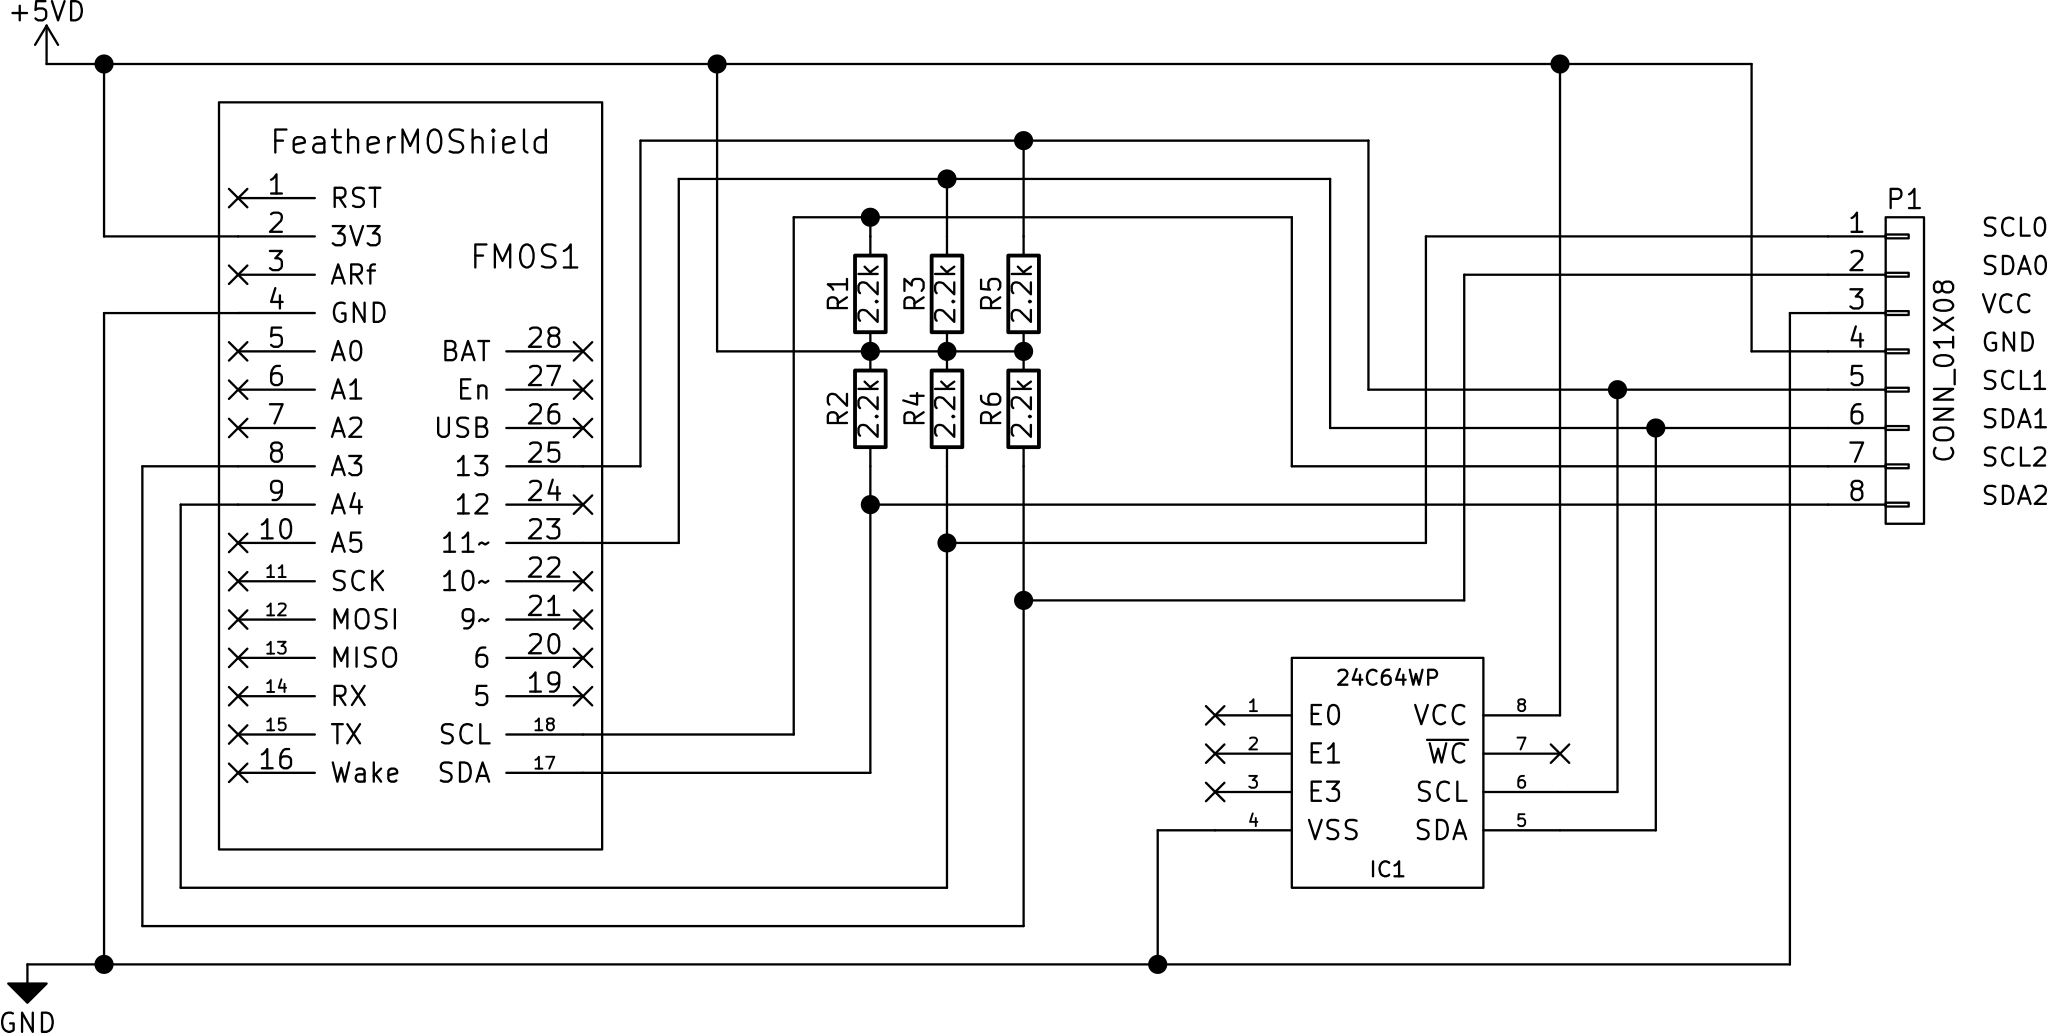
\includegraphics[height=5cm]{../common/images/shield-schematics}
        \caption{Schaltplan}
        \figlabel{shield:schematics}
    \end{subfigure}
    \hfill
    \begin{subfigure}[b]{0.3\textwidth}
        \centering
        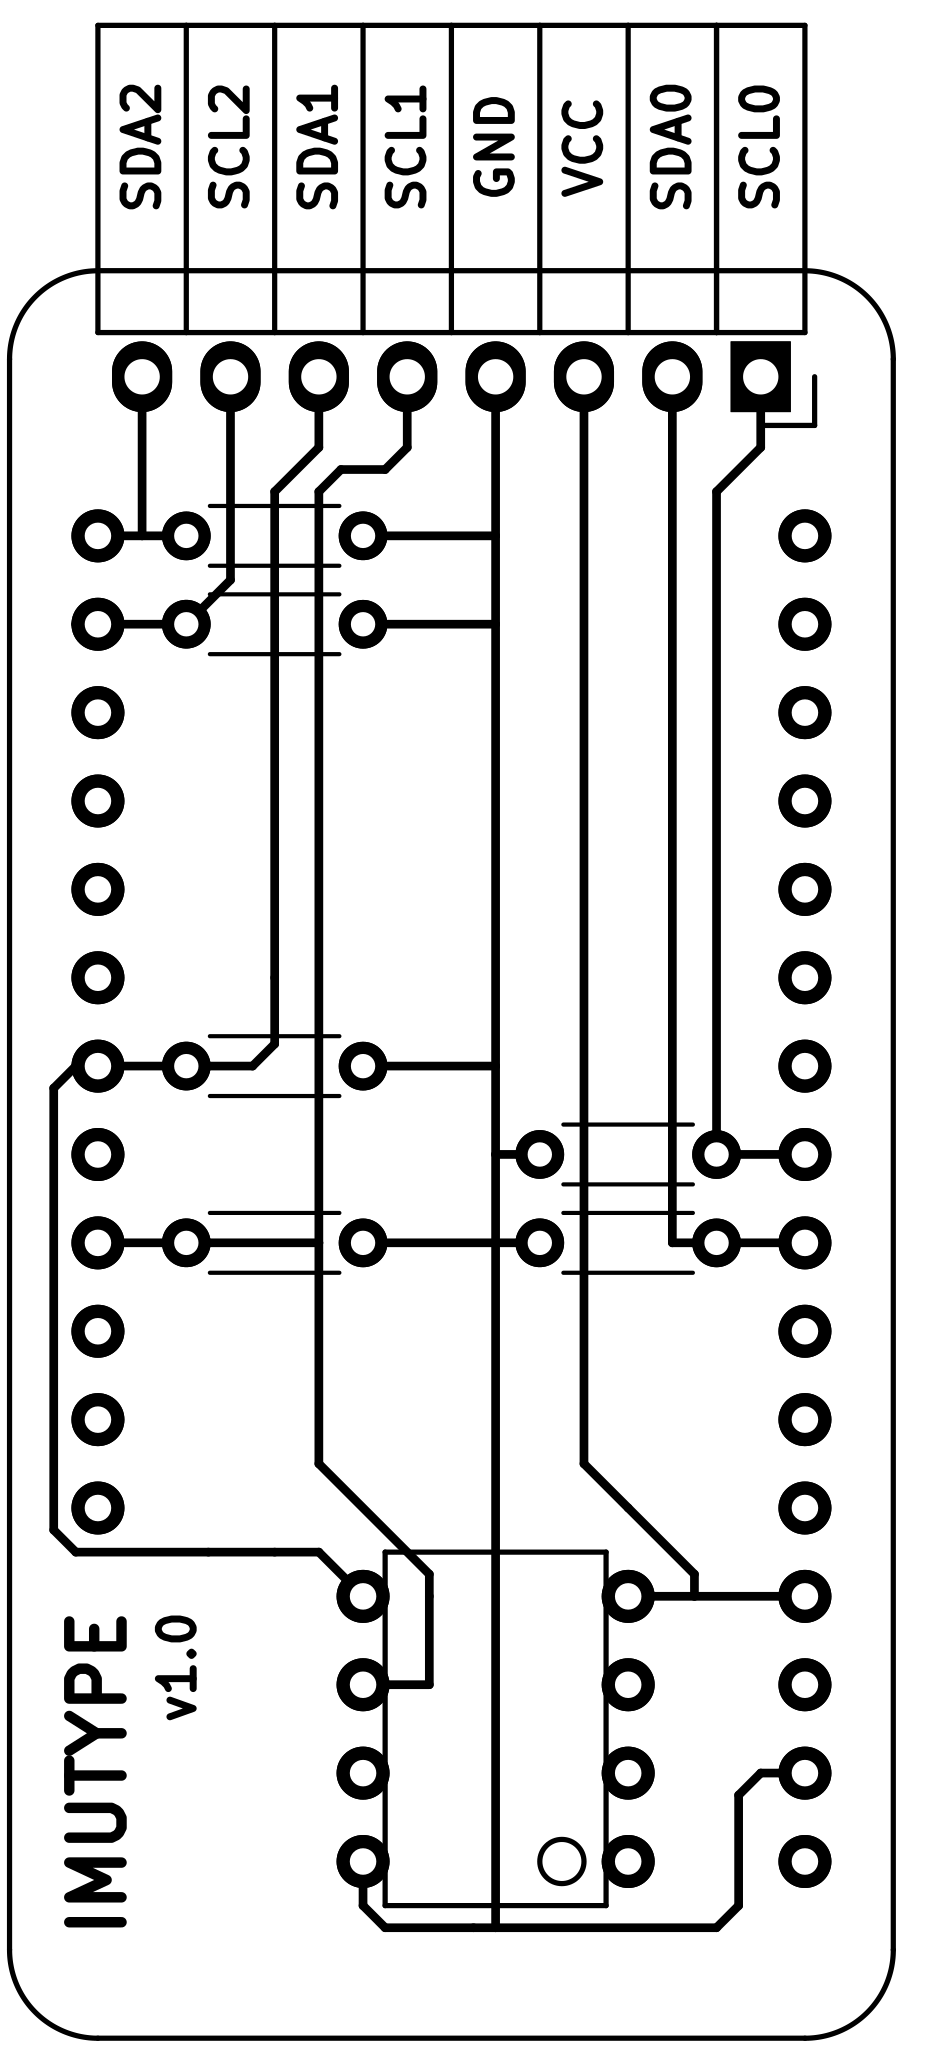
\includegraphics[height=5cm]{../common/images/shield-board}
        \caption{Leiterbahnlayout}
        \figlabel{shield:board}
    \end{subfigure}

    \caption[Schaltplan und Leiterbahnlayout des Shields]{Die Verkabelung der zur Ansteuerung der Sensoren benötigten
    Komponenten erfolgt auf dem ,,Shield'', einer Platine, welche sich auf das
    Featherboard aufstecken lässt (vgl. \figref{photos:shield}).}
    \figlabel{shield}
\end{figure}


In \figref{shield:schematics} sehen wir den Schaltplan für die Verkabelung der
Komponenten am Handgelenk. Nicht enthalten sind die tatsächlichen Sensoren,
diese werden am Ende an die jeweiligen Busse angebracht (VCC, GND, SDA, SCL an
die dazugehörigen Pads auf dem Sensor-Board). Am rechten Rand befindet sich
stattdessen die Buchsenleiste, die SDA und SCL aller Busse sowie VCC und GND
zur Verfügung stellt. Das EEPROM vom Typ \productname{24C64WP} ist an Bus 1
angeschlossen. Zusätzlich enthalten sind die Pull-up-Widerstände, die
erforderlich sind, weil das Featherboard keine integrierten Pull-up-Widerstände
enthält.

Um die Verkabelung einfach zu halten, entwarfen wir einen ,,Shield'' zum
Aufstecken auf das Featherboard. Dieses entspricht dem gezeigten Schaltplan,
und beinhaltet eine Buchsenleiste zum Anstecken des Handschuhs.
\figref{shield:board} zeigt ein mögliches Leiterbahnlayout für diese Schaltung.
Es hat aufgrund der Anordnung der Busse keine Überkreuzungen und benötigt somit
nur eine Kupferschicht. Die Busse sind von links nach rechts in umgekehrter
Reihenfolge angeordnet, dazwischen befinden sich GND und VCC. Die Buchsenleiste
ist ,,oben'', in Handrichtung.

Aus der Anordnung der Busse ergibt sich \tabref{wires}, welche die Zuordnung
der IMUs zu ihrem Bus zeigt, sowie die gewählte Adresskonfiguration. Außerdem
erhält jede IMU eine ID zur späteren Identifizierung der Daten. Auch hier haben
wir darauf geachtet, möglichst wenige Überkreuzungen zu verursachen. Da die
linke und rechte Hand Spiegelbilder sind, aber der gleiche Prozessor und Shield
verwendet werden, haben wir die Reihenfolge der Bus-Zuordnungen umgekehrt. Wie
zu erkennen ist, werden die Busse von rechts nach links an der jeweiligen Hand
angeordnet, statt von innen nach außen.

\begin{table}
    \centering
    \renewcommand{\arraystretch}{1.2}
\begin{tabular}{@{}clllll@{}}
    \toprule
    Hand & IMU & Platzierung & Bus & Adresse & AD0-Pin \\ \midrule
    \multirow{6}{*}{\rotatebox[origin=c]{90}{rechts}} &
      0 & Handrücken        & 2 & 0x28 & low \\
    & 1 & Daumen            & 2 & 0x29 & floating \\
    & 2 & Zeigefinger       & 1 & 0x28 & low \\
    & 3 & Mittelfinger      & 1 & 0x29 & floating \\
    & 4 & Ringfinger        & 0 & 0x28 & low \\
    & 5 & Kleiner Finger    & 0 & 0x29 & floating \\
    \midrule
    \multirow{6}{*}{\rotatebox[origin=c]{90}{links}} &
      6  & Handrücken       & 0 & 0x28 & low \\
    & 7  & Daumen           & 0 & 0x29 & floating \\
    & 8  & Zeigefinger      & 1 & 0x28 & low \\
    & 9  & Mittelfinger     & 1 & 0x29 & floating \\
    & 10 & Ringfinger       & 2 & 0x28 & low \\
    & 11 & Kleiner Finger   & 2 & 0x29 & floating \\
    \bottomrule
\end{tabular}

    \caption{Zuordnung der IMUs zu Positionen an der Hand und den \iic-Bussen
    und "~Adressen.}
    \tablabel{wires}
\end{table}

\section{Befestigung} \seclabel{befestigung}

Besonders für das Ziel der geringen motorischen Einschränkung ist die Wahl der
Befestigungsmethode relevant. Die Testperson muss in der Lage sein, die im
Muskelgedächtnis gespeicherten Bewegungen ohne oder mit nur minimalen
Beeinflussungen auszuführen.

Die Basis-IMU auf dem Handrücken lässt sich am einfachsten auf einem Handschuh
platzieren. Auch vorstellbar ist zum Beispiel ein Clip, welcher sich von der
Handinnenfläche über den Handrücken klemmt. Der erhöhte Produktionsaufwand und
die erschwerte Verkabelung sprachen in unserem Projekt dagegen. Ein schmales
Gummiband um die Hand kam für uns ebenfalls nicht infrage, da dieses stark
gespannt sein müsste, um bei Bewegungen der Hand nicht zu verrutschen, der von
dem Gummiband ausgeübte Druck würde dann jedoch den Tragekomfort
beeinträchtigen.

Besonders wichtig für das Tippen sind die Fingerkuppen, daher haben wir uns
dafür entschieden, diese und das dritte Fingerglied frei zu lassen. Also
befestigen wir die Sensoren am zweiten Fingerglied. Um hier möglichst wenig
Material zwischen die Finger zu bringen, das an den benachbarten Fingern reiben
könnte, nehmen wir ein einfaches Elastikband, und bilden daraus Ringe.  Die
Sensoren kleben wir an der Oberseite auf. Für einen Prototyp ist diese
Konstruktion stabil genug.

% Die an die Testperson angepassten Elastikbänder sind
% zwar so fest, dass sie nicht verrutschen, aber ermöglichen trotzdem noch einen
% hohen Tragekomfort, ohne nach einer längeren Tragzeit abzuschnüren.

Wir verlöteten den \texttt{AD0}-Pin direkt an jedem zweiten Sensor mit
\texttt{GND}. Die vier Kabel leiteten wir am Finger entlang und befestigten sie
mit etwas Faden am fingerlosen Handschuh. So nah an den Fingerspitzen wie
möglich bündelten wir die zusammengehörigen Kabel und verlöteten sie. Dadurch
haben wir die Kabelmenge von 24 auf 8 Kabel reduziert und Gewicht eingespart.
Die 8 übrigen Kabel werden wir zur Steckerleiste geführt, welche auf die
Buchsenleiste des Shields passt. \figref{photos:finished-glove} zeigt den
fertigen Handschuh.

\begin{figure}
    \begin{subfigure}[b]{0.59\textwidth}
        \centering
        \fbox{\includegraphics[height=6cm]{../common/images/glove-sideways}}
        \caption{Der fertige Handschuh}
        \figlabel{photos:finished-glove}
    \end{subfigure}
    \hfill
    \begin{subfigure}[b]{0.4\textwidth}
        \centering
        \fbox{\includegraphics[height=6cm]{../common/images/shield}}
        \caption{Shield und Featherboard}
        \figlabel{photos:shield}
    \end{subfigure}

    \caption[Fotos der Hardwarekomponenten]{Fotos der Hardwarekomponenten.
    Links ist der gesamte Handschuh zu sehen, inklusive der durch Gummiringe an
    den Fingern befestigten IMUs und der Basis-IMU auf dem Handrücken. Der
    Shield ist auf das Featherboard aufgesteckt und durch eine Steckverbindung
    mit dem vorderen Handschuhteil verbunden. Shield und Featherboard (einzeln
    im rechten Bild zu sehen) sind auf einer Manschette am Handgelenk
    befestigt.}
    \figlabel{photos}
\end{figure}

\section{Datenübertragung} \seclabel{uebertragung}

Die erfassten Daten werden vom Mikroprozessor an den Host-PC übertragen. Dies
soll über WLAN, also per Netzwerkprotokoll möglich sein. Zur einfachen
Entwicklung des Systems ist es außerdem wünschenswert, den Handschuh per USB
anzuschließen. Dadurch ist die Verbindung stabil, die Stromversorung
sichergestellt und man muss keine WLAN-Zugangsdaten einpflegen.

Um sowohl die serielle USB-Schnittstelle als auch den netzwerkbasierten Modus
unterstützen zu können, haben wir unser eigenes paketbasiertes Protokoll definiert.
Mithilfe dieses Protokolls können wir die Daten bestimmen, welche übermittelt
werden sollen. Dies hat den Vorteil, dass wir ausschließlich Daten von
Interesse übermitteln und dadurch die Übertragungsgeschindigkeit verbessern.

Paketbasiert bedeutet in unserem Fall, dass wir jede Information in ein
Datenpaket verpacken. Diese werden dann entweder seriell per USB übertragen,
oder unabhängig voneinander per WLAN mit UDP gesendet.

Es gibt in unserem Anwendungsfall 4 verschiedene Arten von Paketen: Header,
IMU Data, Debug Message und Key State Change.

\begin{description}
    \item[Header] Dieses Paket wird immer nach Abschluss des Bootvorganges
        gesendet und beginnt mit einem ,,Magic header'', der willkürlich
        gewählten, festen Bytefolge \texttt{49 D2 C8 CE}. Diese ist hilfreich,
        um zu erkennen, dass es sich tatsächlich um einen Datenstrom vom
        Mikroprozessor handelt. Alle nachfolgenden Bytes auf der seriellen
        Schnittstelle müssen dem in unserem Protokoll formulierten Format
        entsprechen.

        Das Header-Paket beinhaltet die in \tabref{packet-format-header}
        aufgeführten Felder.

        \begin{table}[h]
            \centering
            \begin{tabular}{@{}llll@{}}
                \toprule
                Offset & Länge & Wert & Beschreibung \\ \midrule
                0   & 4 & \texttt{49 D2 C8 CE} & Magic header \\
                4   & 1 & \texttt{03} & Protokollversion \\
                5   & 1 & & Anzahl IMUs \\
                6   & 2 & & Wertebereich Accelerometer \\
                8   & 2 & & Wertebereich Gyroskop \\
                10  & 4 & & Aktuelle Prozessorzeit \\
                14  & 18 & \texttt{00 00 00 \ldots} & Padding auf 32 Byte Länge \\
                \bottomrule
            \end{tabular}
            \caption{Datenformat des Header-Pakets}
            \tablabel{packet-format-header}
        \end{table}

        Die Protokollversion gibt uns die Freiheit, das Protokoll zu erweitern
        und anzupassen, aber mit alten Datensätzen kompatibel zu bleiben.

        Da die Anzahl der IMUs sowie deren Konfiguration hardwareseitig
        festgelegt wird, übertragen wir beides im Header-Paket an den Host,
        sodass dieser die Daten entsprechend korrekt interpretieren kann.
        Ebenso verhält es sich mit den konfigurierten Wertebereichen der
        Sensoren, welche in der späteren Berechnung der tatsächlichen Messwerte
        verwendet werden.
\end{description}

Alle Pakete, die nicht vom Typ Header sind, haben das in \tabref{packet-format}
gezeigte Datenformat.  Die aktuelle Prozessorzeit wird in allen Paketen
übertragen, da es sich um zeitsensible Daten handelt, und die Prozessorzeit die
genaueste Angabe ist, die wir zu einem Datensatz machen können.

\begin{table}[h]
    \centering
    \begin{tabular}{@{}llll@{}}
        \toprule
        Offset & Länge & Wert & Beschreibung \\ \midrule
        0   & 1 & \texttt{C1} & Paketstart-Markierung \\
        1   & 2 & & Pakettyp (s.u.) \\
        2   & 4 & & Aktuelle Prozessorzeit \\
        6 & $l$ & & (Paketinhalt) \\
        $6 + l$ & 1 & \texttt{1C} & Paketende-Markierung \\
        \bottomrule
    \end{tabular}
    \caption{Datenformat aller Pakete, die nicht vom Typ Header sind.}
    \tablabel{packet-format}
\end{table}

Alle Ganzzahl-Werte werden in Little Endian gesendet. Dies ist in
Netz\-werk\-pro\-to\-kol\-len zwar unüblich, da aber die Sensoren die Daten in
dieser Byte-Reihenfolge bereitstellen, ersparen wir uns ein Umsortieren auf dem
Mikroprozessor.

\begin{description}
    \item[Debug Message (\texttt{0x01})]
        Dieser Pakettyp beinhaltet eine Nachricht zur Anzeige auf dem Host, zum
        Zwecke der Entwicklung, um zum Beispiel über die erfolgte Initialisierung
        einer IMU zu informieren. Der Paketinhalt besteht aus 2 Bytes
        Nachrichten-Code (arbiträr), 2 Bytes Textlänge, und dem Text der
        Nachricht, in ASCII codiert.

    \item[IMU Data (\texttt{0x02})]
        Das wohl wichtigste Paket beinhaltet die aktuellen Messwerte einer IMU.
        Der Paketinhalt ist 20 Bytes lang:

        \begin{itemize}[noitemsep]
            \item 6 Bytes lineare Beschleunigung,
            \item 6 Bytes Winkelgeschwindigkeit und
            \item 8 Bytes Orientierung (Quaternion).
        \end{itemize}


        Wir senden keine Fließkommawerte, da die Sensoren Ganzzahlwerte
        bereitstellen, welche unter Berücksichtigung des eingestellten
        Wertebereiches zu Dezimalzahlen in Standardeinheiten umgerechnet werden
        können. Diese Umrechnung findet der Einfachheit halber erst auf dem
        Host-PC statt.  Für die Vektoren errechnet sich der tatsächliche Wert
        durch folgende Formel:

        $$V_{real} = \frac{V_{integer}}{2^{15} \cdot \text{range}}$$

        Den Wertebereich (range) erhält man aus dem Header-Paket.

        Quaternionen sind normalisiert und einheitslos, daher werden sie im
        Gegensatz zu den Vektoren ohne Verwendung eines Wertebereichs
        errechnet:

        $$Q = \frac{Q_{integer}}{2^{14}}$$

    \item[Key State Change (\texttt{0x03})]
        Mit diesem Paket ist der Mikroprozessor in der Lage, eine Taste zu
        simulieren, etwa wenn Buttons am Handschuh befestigt sind. Wir haben
        diese Funktion in anfänglichen Experimenten verwendet, um die
        Funktionalität des Handschuhs zu testen. In Zukunft könnte man
        Funktionstasten in den Handschuh integrieren, etwa um zwischen
        verschiedenen Modi zu wechseln.

        Das Paket beinhaltet neben den üblichen Feldern lediglich einen Key
        Code von 2 Bytes, sowie 1 Byte Tastenzustand (\texttt{0x01} für gedrückt,
        ansonsten \texttt{0x00}).
\end{description}

\section{Datenverarbeitung}

Die Software auf dem Host-PC ist komplett in Python implementiert. Hierfür
kommen hauptsächlich folgende Bibliotheken zum Einsatz:

\begin{itemize}
    \item \texttt{NumPy} \citep{numpy} für die Datenverarbeitung mit Vektoren und
        mehrdimensionalen Matrizen
    \item \texttt{Theano} \citep{theano} und
        \texttt{Lasagne}~\cite{web:lasagne} zur Modellierung und Berechnung der
        neuronalen Netze
    \item \texttt{Matplotlib} \citep{matplotlib} zur Datenanalyse,
        Visualisierung der rohen und vorverarbeiteten Daten, Zeichnen der
        Lernfortschrittsgraphen
    \item \texttt{ROS}~\cite{web:ros} zur Verknüpfung eigenständiger Komponenten über
        wohldefinierte Kommunikationskanäle, sogenannte ,,topics'', dies beinhaltet
        \texttt{rosbag} als Datenspeicher für Lerndaten
\end{itemize}

Die Verwendung von NumPy ist unverzichtbar, da insbesondere
Theano darauf aufbaut. Numpy ist eine weitverbreitete Bibliothek für
die wissenschaftliche Datenverarbeitung in Python. Sie ist einfach zu benutzen,
stark optimiert und auf die Verarbeitung hochdimensionaler Daten ausgelegt.

Theano baut hierauf auf und stellt Funktionen bereit, mit denen
komplexe Rechenoperationen deklariert und dann auf unterschiedliche Arten
ausgeführt werden können. Prinzipiell definiert man mit Theano zuerst den
mathematischen Zusammenhang zwischen verschiedenen Symbolen und lässt sich dann
eine Funktion generieren, welche diese Zusammenhänge auflöst und mitunter sehr
komplexe Berechnungen durchführt. Theano kann konfiguriert werden, diese
Funktion zum Beispiel just-in-time für eine oder mehrere CPUs, oder auch GPUs,
zu kompilieren. Dadurch werden die Berechnungen sehr performant.

Lasagne ist eine Bibliothek, die es vereinfacht, neuronale Netze in Theano zu
modellieren. Dadurch erspart man sich die komplexe Deklaration der
mathematischen Modellierung eines Netzes mit Matrizen, und kombiniert nur
einzelne Netzwerkschichten mit entsprechender Konfiguration zu einem
Gesamtnetz. Dies beschleunigt die Entwicklung extrem und erlaubt es, sehr
flexibel mit der Netzwerkkonfiguration zu experimentieren.

Wir verwenden ROS, das ,,Robot Operating System'' aus verschiedenen Gründen.
ROS ist eine Sammlung von Bibliotheken und Programmen, welche zur Entwicklung
von Robotersystemen in der Forschung dienen. Den Kern bildet hierbei ein
IPC-System (\fremdwort{interprocess communication}), das mithilfe sogenannter
,,topics'' Kommunikation zwischen Prozessen über fest definierte Schnittstellen
erlaubt.

Zunächst benutzten wir diesen Mechanismus der Kommunikation für jeden
Verarbeitungsschritt, etwa auch zwischen Preprocessing und Sampling. Da dies
jedoch einen gewissen Mehraufwand mit sich bringt und Verzögerungen einführt,
entschieden wir uns dazu, nur noch bei einigen Verbindungen ROS-Topics
einzusetzen. Am Ende nutzen wir ROS für die Übermittlung der Rohdaten sowie der
tatsächlichen Tastenanschläge zum Preprocessing, und für die Ausgabe des
Klassifikators im Anwendungsmodus. Alle anderen Verbindungen ersetzten wir
durch Python Koroutinen (\fremdwort{coroutines}), welche ein ähnlich
gekapseltes Programmieren ermöglichen wie die \fremdwort{topic callbacks} von
ROS.

Ein großer Vorteil der Verwendung von ROS für die Rohdaten ist, dass wir
\emph{rosbag} verwenden können. Hierbei handelt es sich um ein Tool, das die
Nachrichten eines oder mehrerer Topics aufzeichnet und später abspielt.
Dadurch konnten wir Lerndaten aufzeichnen, und später mit verschiedenen
Parametern und Algorithmen anhand dieser Daten lernen.  Wir spielen dabei die
Aufzeichnung nicht ab, sondern verwenden die Python-Bibliothek von
rosbag direkt, um die Daten auszulesen.

Es erwies sich als hilfreich, die gesamte Pipeline bis zum Schritt ,,Sampling''
(vgl. \figref{overview}) vom Aufruf des Lernprozesses zu trennen. Das
Zwischenergebnis, ein großes NumPy-Array mit allen Samples, speichern wir in
eine eigene Datei. Wir schrieben uns einige Tools, um diese Samples analysieren
zu können, einige dieser Visualisierungen zeigen wir im \chapref{bewertung}.

Für andere Analysen waren die in ROS enthaltenen Tools sehr hilfreich.
Insbesondere RViz, ein 3D-Visualisierungs-Programm für ROS, ist gut geeignet,
um Fehler bei der Entwicklung zu erkennen. Hauptsächlich nutzte uns RViz beim
Entwickeln der Vorverarbeitung der Quaternionen.

Für die Konfiguration des gesamten Prozesses verwenden wir eine zentrale
Konfigurationsdatei. Diese wird im YAML-Format geschrieben und enthält alle
Parameter, die für den Aufbau des Experiments relevant sind. \lstref{config}
zeigt eine beispielhafte Ausprägung dieser Konfigurationsdatei. Die Bedeutung
der einzelnen Einstellungen wird in \cite{caro} erläutert.  Hervorheben möchte
ich an dieser Stelle, dass wir für jedes Experiment eine eigene
Konfigurationsdatei anlegen können, und somit jedes Experiment nachvollziehbar
und wiederholbar wird. Alle Softwareteile laden beim Start die angegebene
Konfiguration und benutzen die für den jeweiligen Verarbeitungsschritt
relevanten Teile daraus.  Ins jeweilige Verzeichnis des Experiments, neben die
Konfigurationsdatei, werden auch alle Eingabedaten (ROS-Bag),
Zwischenergebnisse (NumPy-Array) und Ausgaben (Lernfortschritt-Statistiken,
generierte Graphen, \ldots) abgespeichert.

\begin{listing}
    \inputminted{yaml}{../common/code/config.yaml}
    \caption[Beispiel für eine Konfigurationsdatei]{Beispiel für eine Konfigurationsdatei. Wir verwenden diese, um die
    Initialisierung aller Softwarekomponenten zu beeinflussen. Dies beinhaltet
    die Vorverarbeitung, die mit Lasagne modellierte Netzwerkarchitektur, das
    Lernverhalten und den Anwendungsmodus.}
    \lstlabel{config}
\end{listing}

\section{Einbindung als Tastatur ins Betriebssystem}

Vorerst unterstützt unser System nur die Einbindung unter GNU/Linux, sodass die
generierten Tastendrücke auch tatsächlich als solche benutzt werden können.
Verwendet wird dafür das Input-Event-System \emph{evdev}, welches über
die dazugehörige Python-Bibliothek sehr einfach zu integrieren ist.

\begin{listing}
    \inputminted{python}{../common/code/evdev.py}
    \caption[Beispiel für die Verwendung von \texttt{python-evdev}]{Beispiel
    für die Verwendung von \texttt{python-evdev} zur Emulation von
    Tastendrücken in einem Linux-System.  Das \texttt{event} stammt hierbei vom
    ROS-Topic \texttt{/predicted\_key\_events}, welches die vom Klassifikator
    erkannten Tastendrücke übermittelt.}
    \lstlabel{evdev}
\end{listing}

Diese Verwendung von \texttt{python-evdev} ist in \lstref{evdev} skizziert.
Eine ähnliche Integration wäre für andere Betriebssysteme selbstverständlich
ebenfalls denkbar.

% vim: tw=79

\chapter{Maschinelles Lernen} \chaplabel{ml}

In diesem Kapitel möchte ich kurz das Vorgehen und die Ergebnisse des
maschinellen Lernens beschreiben, um eine vollständige Verständlichkeit des
Gesamtprojektes zu ermöglichen. Ich werde jedoch nicht alle Details beleuchten,
da dies außerhalb des Themas dieser Arbeit liegt. Die genaue Ausarbeitung
dieser Aspekte sind Inhalt der Bachelorarbeit von Carolin \citet{caro}, und
dort nachzulesen.

\section{Überblick}

In \figref{overview} habe ich bereits alle Komponenten des maschinellen Lernens
in unserem Projekt vorgestellt. Angefangen im \fremdwort{Preprocessing} werden
die Rohdaten von den Sensoren und der Tastatur vorverarbeitet. Aus diesem
Datenstrom werden im \fremdwort{Sampling} sogenannte Samples extrahiert, also
unabhängige Datensätze, welche jeweils ein Lernbeispiel beinhalten. Im
\fremdwort{Learning} wird der gewählte Algorithmus angepasst, indem ihm
Lernbeispiele vorgestellt werden. Das gelernte Modell wird gespeichert und kann
dann in \fremdwort{Apply Network} direkt mit den vorverarbeiteten Daten
angewendet werden, um eine Vorhersage (\fremdwort{prediction}) zu generieren.

Die wichtigste Entscheidung ist die Wahl des ML-Algorithmus. Da wir Datensätze
mit den dazugehörigen tatsächlichen Ergebnissen (Tastaturanschläge)
aufzeichnen, können wir einen Algorithmus des überwachten Lernens wählen. Wir
entscheiden uns für ein neuronales Netzwerk, da diese in der Lage sind sehr
komplexe Zusammenhänge zu erlernen, und wir flexibel das Netzlayout und die
Parameter konfigurieren und optimieren können. Auch sind neuronale Netze,
sobald sie trainiert wurden, sehr effizient anzuwenden, was in unserer
Echtzeitanwendung wichtig ist.

Bei den neuronalen Netzen gibt es zahlreiche Varianten, die sich alle in ihrem
Aufbau und damit in ihrer Funktion unterscheiden. Da wir Zeitfolgen lernen
wollen, experimentierten wir zuerst mit einfachen rekurrenten Netzen
\citep{elman-rnn}. Hier traten jedoch Probleme auf, da unseren Daten
unausgeglichenen sind: Der Anteil der Zeit, in der gerade eine Taste gedrückt
wird, ist verhältnismäßig zum Rest sehr gering. Außerdem beobachten wir das
\fremdwort{Vanishing Gradient Problem} \citep{hochreiter-vanishing-gradient},
also die Problematik, dass die vorderen Schichten im Netz nur sehr langsam
angepasst werden, weil rekurrente Netze sehr tief sind.

Stattdessen wählten wir ein \fremdwort{Convolutional Neural Network}
\citep[CNN;][]{cnn_orig}. Dieser Netztyp wird häufig in der Bilderkennung
eingesetzt, da er in der Lage ist, mehrdimensionale Muster zu unterscheiden.
Dies geschieht durch eine Aneinanderreihung mehrerer Convolution-Pooling
Schichtpaare. In der Convolution werden mithilfe von Filtern (ähnlich den
Kerneln in der Bildverarbeitung) verschiedene Features extrahiert. Das
markanteste lokale Feature wird im Pooling ermittelt, wobei die Größe des
Datensatzes verringert wird. Somit reduziert sich nach einigen Wiederholungen
die Datenmenge auf die ,,interessanten'' Informationen aus den Originaldaten.
Diese können dann mit einer oder mehreren vollständig verknüpften
Netzwerkschichten klassifiziert werden.

\section{Experimente}

Zur Bewertung des Systems führten wir verschiedene Experimente durch, in denen
wir die Brauchbarkeit der Hardware und des ML-Ansatzes testeten. Diese
Experimente lassen sich in 4 Phasen einteilen:

\begin{description}
    \item[Vorbereitung]
        Zunächst entwickelten wir unter Verwendung von Dummy-Aufzeichnungen das
        gesamte Softwaresystem, um alle Einzelschritte der kompletten Pipeline
        und deren Zusammenspiel zu testen.

    \item[Phase 1: Erkennen einer Taste]
        Hier zeichneten wir einen Datensatz auf, in welchem der Proband
        ausschließlich 2 Tasten, \keyboard{N} und \keyboard{H} drückte. Unser
        Ziel war es, den Datensatz zunächst manuell zu analysieren, und
        anschließend automatisch die Tastendrücke erkennen. Dabei wollten wir
        untersuchen, ob der gewählte ML-Algorithmus in der Lage war, anhand der
        Daten Tastendrücke zu erkennen und unter den benachbarten Tasten zu
        unterscheiden.

    \item[Phase 2: Differenzieren verschiedener Tasten]
        In dieser Phase weiteten wir die Anzahl der Tasten von 2 auf 10 aus und
        benutzten somit auch mehrere Finger (Daumen, Zeigefinger und
        Mittelfinger). Die dabei aufgetretenen Probleme beschreibe ich in
        \secref{probleme}.

    \item[Phase 3: Flüssiges Schreiben]
        Diese Phase haben wir noch nicht begonnen, sie wird darauf abzielen
        alle Tasten einer Hand ohne Pausen zwischen den Tastenanschlägen
        benutzen zu können.
\end{description}

\section{Ergebnisse}

In der ersten Phase bemerkten wir bereits, dass unser ursprünglicher Ansatz mit
dem rekurrenten Netz nicht geeignet war, und wechselten zum CNN.  Es
kristallisierte sich heraus, dass ein CNN in der Lage ist, die Fingerbewegungen
für das Drücken einer Taste zu erkennen und in einem gewissen Maße auch der
korrekten Taste zuzuordnen. In der ersten Phase erreichten wir eine
Prädiktionsgenauigkeit von knapp 97\%.

In der zweiten Phase wurde uns jedoch bewusst, dass die Aufgabe recht komplex
ist und noch einiger Verbesserungen bedarf. Ein erstes Experiment in dieser
Phase war weitaus weniger erfolgreich als erhofft. Das Netz war in der Lage,
zwischen einigen der 10 Tasten zu differenzieren, allerdings wurden
\keyboard{H}, \keyboard{J}, \keyboard{\spacebar} und $\emptyset$ (,,keine Taste
gedrückt'') nicht voneinander unterschieden. Wir begründeten dies damit, dass
meine Finger in der Ruheposition auf diesen Tasten liegen, und die Bewegungen
für diese Tasten nur relativ klein sind.

In einer zweiten Wiederholung des Experimentes mit gleichen Daten hatten wir
mehr Glück, nach einiger Zeit wurden auch diese problematischen Tasten erkannt,
wenn auch nicht mit der gleichen Genauigkeit wie die anderen Tasten. Insgesamt
erreichte die Klassifikation eine Genauigkeit von 85\%. Dieses Ergebnis ist
recht zufriedenstellend, wenn auch noch ausbaufähig.

Für die nächste Phase, in welcher das flüssige Schreiben gelernt werden soll,
müssen noch einige Verbesserungen durchgeführt werden. Vorschläge hierfür
werden in der Arbeit von Carolin \citet*{caro} geschildert.

% vim: tw=79

\chapter{Bewertung} \chaplabel{bewertung}

In diesem Kapitel bewerte ich den nach unserem Design umgesetzten
Datenhandschuh und das Gesamtsystem. Ich gehe dabei auf die Datenqualität ein,
und stelle Probleme vor, die diese negativ beeinflusst haben. Danach bewerte
ich, ob wir unsere Designziele aus \chapref{ziele} erreicht haben, und erwähne
mögliche Verbesserungen, die wir am System noch erkannt haben.

\section{Datenqualität} \seclabel{datenqualitaet}

Die vom Handschuh ermittelten Daten sind von ausreichender Qualität, wenn man
an ihnen unterschiedliche Tastenanschläge erkennen kann. Nur dann ist auch ein
ML-Al\-go\-rith\-mus in der Lage, diese Erkennung ebenfalls durchzuführen.

\begin{figure}
    \includegraphics[width=\textwidth]{../common/images/plot-samples-2x2}
    \caption[Einzelne Samples der Tastendrücke N und H]{Mehrere Wiederholungen
    der Tasten N und H, überlagert zum Zeitpunkt des Drückens der Taste
    (Mittellinie). Gezeichnet sind zur einfacheren Visualiserung der relative
    Pitch"~ und Yaw-Winkel des rechten Zeigefingers. Der Zeigefinger liegt
    zwischen den Tastendrücken in Ruheposition auf der Taste H.}
    \figlabel{plot-samples-2x2}
\end{figure}

\figref{plot-samples-2x2} zeigt die extrahierten, vorverarbeiteten Daten aus
Phase 1. Auf der linken Seite wurde die Taste \keyboard{N} und auf der rechen
Seite die Taste \keyboard{H} gedrückt. In den oberen Graphen ist der
Pitch-Winkel, unten der Yaw-Winkel des rechten Zeigefingers relativ zur
Handbasis aufgezeichnet.  Entlang der x-Achse ist die Zeit vor und nach dem
Tastenanschlag aufgeführt, zum Zeitpunkt des Tastenanschlages ist eine
Hilfslinie im Graphen eingezeichnet.  Jedes Sample (also jeder Tastendruck)
tritt als einzelne Linie im Graphen auf. Anhand diesen Samples wird das Netz
trainiert\footnote{Tatsächlich benutzen wir für das Training die Quaternionen,
wir zeigen hier die Euler-Winkel, da diese einfacher zu verstehen sind.}.

Die Unterschiede in den Bewegungsmustern für die verschiedenen Tastenanschläge
sind hier gut zu erkennen. Wir stellen fest, dass sich alle Samples innerhalb
des gleichen Graphen bis auf einige Ausnahmen sehr ähneln -- dies ist wichtig
für die Erkennung eines Musters.  Die Amplitude des Ausschlages ist jeweils
vergleichbar, einzig der y-Offset ist teilweise von Sample zu Sample
unterschiedlich (gut erkennbar im N-Yaw-Graphen).

\begin{figure}[p]
    \centering
    \advance\leftskip-2cm
    \includegraphics[width=17cm]{../common/images/graphs-average}
    \caption[Mittel aller Samples verschiedener Tastenanschläge aus
    Phase~2]{Mittel aller Samples verschiedener Tastenanschläge aus Phase~2,
    aufgeteilt nach Eingabewert und Sensor. Auf der x-Achse ist die Zeit vor
    und nach dem Tastenanschlag aufgetragen, die y-Achse zeigt den jeweiligen
    Eingabewert (v.o.n.u Quaternion w, x, y, z, Accelerometer x, y, z in
    $m/s^2$).  Für jede Taste wurden etwa 150 Samples aufgezeichnet.}
    \figlabel{graphs-average}
\end{figure}

\figref{graphs-average} enthält viele verschiedene Graphen, welche aus den
Aufzeichnungen für Phase 2 (siehe \chapref{ml}) extrahiert wurden. Für einen
Teil der Tasten\footnote{Phase 2 enthält 10 verschiedene Tasten, wir zeigen zur
Übersicht nur 6 davon.} werden hier sowohl die Quaternionen, als auch die
Accelerometerdaten über die Zeit aufgezeichnet. Der Tastenanschlag liegt nun
bei drei Vierteln des gezeichneten Zeitfensters. Jeder Subgraph enthält 6
Kurven, jeweils eine für jeden der Sensoren der rechten Hand. Die einzelne
Kurve ist dabei das Mittel aller für diesen Sensor, Tastenanschlag und
Eingabewert ermittelten Samples.

Für jede der gezeigten Tasten ist in diesen Graphen ein eindeutiges Muster
erkennbar. Beispielsweise sind sich die Muster der Tasten \keyboard{T} und
\keyboard{Y} sehr ähnlich, unterscheiden sich jedoch im Ausschlag der
z-Komponente der Quaternion des rechten Zeigefingers. Dass sich die Muster für
diese Tasten grundsätzlich ähnlich sind, ist verständlich, da sie direkt
benachbart sind, und der Zeigefinger für beide Tasten eine Bewegung nach oben
links von der Ruheposition aus machen muss.

Ein anders Beispiel sind die Tasten \keyboard{H} und \keyboard{J}. Diese
unterscheiden sich auf den ersten Blick nur geringfügig im Muster, es wird fast
keine Änderung an der Orientierung der Sensoren festgestellt. Das liegt daran,
dass in Ruheposition des Probanden der Zeige- und Mittelfinger auf diesen
Tasten liegen, und somit kaum eine Bewegung durchgeführt werden muss. Bei
genauerer Betrachtung stellt man jedoch fest, dass der y- und z-Ausschlag des
Accelerometers von verschiedenen Sensoren stammt, das \keyboard{H} wird also
eindeutig mit dem Zeigefinger betätigt und das \keyboard{J} mit dem
Mittelfinger.

Wir sind grundsätzlich mit der Qualität dieser Daten sehr zufrieden und halten
sie für geeignet, um damit eine Klassifizierung durchzuführen. Zu beachten ist
aber, dass diese Daten schon vorverarbeitet worden sind. Einige der
nachfolgend genannten Probleme wurden in der Vorverarbeitung dabei bereits
behoben.

Es handelt sich bei den gezeigten um im Laborversuch gewonnene Daten. Reale
Daten werden sicher noch ungenauer und uneindeutiger, wir hoffen hier mit
weiteren Verbesserungen der Vorverarbeitungsmethoden gegensteuern zu können und
mehr Eindeutigkeit zu erreichen.

\section{Probleme} \seclabel{probleme}

Im folgenden zeige ich die Probleme auf, welche wir im Laufe unserer Arbeit festgestellt
haben.

\subsection{Gyro clipping}

Im Fusionsmodus, den wir für die Berechnung der Quaternionen aktiviert haben,
steuert die BNO intern die Sensorkonfiguration, sodass sich diese nicht mehr
von außen festlegen lässt, wie es etwa im Rohdaten-Modus der Fall wäre.
Außerdem übernimmt der Fusionsalgorithmus die Kontrolle über die initiale
Kalibrierung der Sensoren und führt Selbsttests und Echtzeitkalibrierungen
durch.

Leider können wir einige Probleme mit dem Fusionsalgorithmus der BNO055
feststellen\footnote{Im Adafruit Forum gibt es eine lange Diskussion zu
verschiedenen Problemen, die andere Benutzer mit der BNO055 erfahren haben,
darunter auch die hier beschriebenen.
\url{https://forums.adafruit.com/viewtopic.php?f=19&t=78459}}. So ist das
Gyroskop fest auf einen Wertebereich von $\SI{\pm500}{deg/s}$ eingestellt, man
kann hierauf keinen Einfluss nehmen. Dreht man den Sensor schneller als dieses
Limit, wird der Wert abgeschnitten, und die Integration der Geschwindigkeit
liefert eine falsche Orientierung. Diese schnellen Bewegungen treten bei
flüssigem Tippen auf.

Wir konnten dies nachstellen, indem wir den Sensor senkrecht platzierten und
von dort schnell in die Waagerechte drehten. Die berechnete Quaternion kommt
dann nicht ganz der Drehung hinterher, es beinhaltet dann Fehler in der Pitch-
und Roll-Komponente.

Eine mögliche Lösung hierfür wird zusammen mit dem folgenden Problem im
nächsten Abschnitt diskutiert.

\subsection{Heading drift}

Ein weiteres Problem ist eine Ungenauigkeit des Headings, also der horizontalen
Ausrichtung. Nach ruckartigen Bewegungen in nicht-waagerechter Orientierung
verliert der Sensor seine Ausrichtung nach Norden. Wir vermuten, dass dies an
der Konfiguration des Kalman-Filters liegt\footnote{Es ist nicht im Datenblatt
der BNO055 spezifiziert, dass es sich bei dem Fusionsalgorithmus um einen
Kalman-Filter handelt, Benutzer ,,Richart100'' im ,,Chief Delphi''-Forum legt
diese Vermutung jedoch nahe: ,,The on-board fusion algorithm, although
unspecified, is likely a Kalman filter variant.''
(\url{https://www.chiefdelphi.com/forums/showthread.php?t=141100}, entnommen am
31.05.2017)}. Dieser bewertet die Genauigkeit des Gyroskopes höher als die des
Magnetometers, vermutlich da das Magnetometer von außen durch Veränderungen im
Magnetfeld beeinflussbar ist. Die Abweichung betrifft nur das Heading, also die
Komponente, die nicht durch den vom Accelerometer gemessenen Gravitationsvektor
korrigiert werden kann.

Diese Abweichung in der Ausrichtung bleibt auch über längere Zeit bestehen,
selbst bei Bewegung des Sensors. Dies erschwert lange Aufzeichnungen mit dem
Handschuh, da die gemessenen Quaternionen zwischendurch ,,verrutschen'' können
und die Samples uneindeutig werden.

Um die Probleme mit dem Gyroskop und dem Drift zu lösen, probieren wir den
Fusionsalgorithmus von \citet{madgwick} aus. Hierfür betreiben wir die BNO055
im Fusionsmodus, lesen aber auch die Rohdaten von Accelerometer, Gyroskop und
Magnetometer aus. Die Rohdaten lassen wir vom Madgwick-Algorithmus in eine
Orientierung umwandeln und vergleichen diese mit der Ausgabe des internen
Fusionsalgorithmus, indem wir beide zu Euler-Winkeln konvertieren und über die
Zeit zeichnen. Die Konvertierung in Euler-Winkel ermöglicht es uns, zwischen
der horizontalen und vertikalen Ausrichtung zu unterscheiden.

Das Ergebnis ist in \figref{madgwick} zu sehen. Wir erkennen, dass die
Algorithmen grundsätzlich sehr ähnliche Ergebnisse liefern.

\begin{figure}
    \includegraphics[width=\textwidth]{../data/heading/heading}
    \caption[Interner Fusionsalgorithmus der BNO055 und Madgwick-Algorithmus im
    Vergleich]{Interner Fusionsalgorithmus der BNO055 und Madgwick-Algorithmus
    im Vergleich. Gezeigt sind Rohdaten des Gyroskops (in
    \si{\radian\per\second}) sowie Euler-Winkel der
    Orientierung (in \si{\radian}).}
    \figlabel{madgwick}
\end{figure}

Im unteren Graphen sehen wir, dass die horizontale Ausrichtung nach den
Bewegungsphasen beim Madgwick-Algorithmus (orange) sich immer wieder dem
Initialwert annähert. Der interne Algorithmus weist hier stattdessen den
beschriebenen Drift auf -- nach 200 Sekunden ist das Heading um knapp
\SI{1}{\radian} zu niedrig, und korrigiert sich nicht wieder.

Der Madgwick-Algorithmus konvergiert jedoch viel langsamer zur korrekten
vertikalen Orientierung, wenn er aufgrund schneller Rotation eine Differenz
zwischen Gravitationsrichtung und gemessener Ausrichtung erkennt.  Dies lässt
sich besonders gut im dritten Graphen erkennen. Teilweise dauert es bis zu 10
Sekunden, bis sich der Wert an den des internen Algorithmus annähert.

Diese Konvergenz lässt sich durch Anpassung des ,,Gain''-Parameters
beschleunigen, jedoch rät Madgwick davon ab, da es das Rauschen verstärkt.  Das
konnten wir leicht überprüfen, die Ausrichtung fängt mit höherem Gain-Wert an
zu zittern. Dies ließe sich eventuell korrigieren, indem man den Wertebereich
der Sensoren erhöht, und somit die Sensitivität verringert. Allerdings müssten
wir dafür den Fusionsmodus deaktivieren und würden die automatische
Echtzeit-Selbstkalibrierung des Sensors verlieren.

% \begin{itemize}
%     \item gyro clippt bei 500 deg/s
%     \item aus senkrechter zurück in waagerechte ist schwer
%     \item Problem:
%     \item es gibt einen alternative algorithmus von Madgwick
%     \item der soll das angeblich können
% \end{itemize}
%

\subsection{Robustheit}

Unser Prototyp erwies sich nicht als besonders langlebig. Nach einigen
Experimenten brachen teilweise die Lötstellen auf, da sie durch die
Handbewegungen vielen Biegungszyklen ausgesetzt waren. Dies ist jedoch
lediglich ein Problem des Prototyps, und keine allgemeine Einschränkung. Einige
Zugentlastungen, eine einteilige Bauweise ohne Steckverbindungen,
eingeschweißte Sensoren sowie mehradrige Kabelverbindungen würden die
Robustheit des Handschuhs deutlich erhöhen.

\subsection{Verwendung einer Laptop-Tastatur}

In unseren Versuchen haben wir die in einen Laptop eingebaute Tastatur
verwendet, welche im Vergleich zu Standard-Tastaturen relativ flach ist.
Dadurch ist die Änderung der Orientierung für einige Tasten sehr gering, es
handelt sich dabei um jene Tasten, auf denen die Finger in Ruheposition liegen
(\keyboard{H}, \keyboard{J}, \keyboard{\spacebar}). Der Algorithmus hat es
dementsprechend schwer, diese Tasten richtig zu klassifizieren, und verwechselt
sie ebenfalls mit der Klasse $\emptyset$. Erst in einer Wiederholung des
Experiments lernte der Algorithmus, diese Tasten zu unterschieden werden,
jedoch mit wesentlich geringerer Genauigkeit als die anderen Tasten. Vermutlich
liegt dieses andere Ergebnis an einer zufällig besseren Initialisierung der
Parameter im Netz.

Die Verwendung einer Tastatur mit genügend Tastenhub würde sicherlich
bessere Ergebnisse erzielen. Außerdem erkennt man, wie in
\figref{graphs-average} gesehen, an den Beschleunigungsdaten Unterschiede. Es
wäre daher ebenfalls gut, den Klassifikator anzupassen, sodass er ebenfalls
die Rohdaten des Accelerometers verwendet.

\section{Sekundäre Designziele}

In diesem Abschnitt gehe ich auf die im \chapref{ziele} vorgestellten Ziele ein
und bewerte, inwieweit wir diese Ziele erfüllt haben. Das primäre Designziel,
charakteristische Werte zu extrahieren, haben wir bereits in
\secref{datenqualitaet} bewertet, und festgestellt, dass die Auswahl und
Qualität der Daten unseren Anforderungen entsprechen.

\subsection{Performance}

\begin{figure}
    \centering
    \includegraphics[width=10cm]{../common/images/delay}
    \caption[Messung der Verzögerung der IMU-Daten]{Messung der Verzögerung der IMU-Daten anhand der z-Komponente der
    Beschleunigung. Die IMU wird zusammen mit der Taste heruntergedrückt. Der
    dazugehörige Ausschlag des Accelerometers wird erst einige Zeit (hier
    \SI{18.6}{\milli\second}) nach dem Tastendruck (Zeitpunkt 0) registriert.
    Im Schnitt ergibt sich eine Verzögerung von rund \SI{15}{\milli\second}.}
    \figlabel{performance}
\end{figure}

Bezüglich der Performance haben wir unser Ziel, die angestrebte Datenrate von
\SI{100}{Hz}, fast erreicht. In unserem Messungen ermittelten wir eine
durchschnittliche Datenrate von rund \SI{90}{Hz}.

Die Verzögerung in der Datenübertragung von den Sensoren bis zum Host-PC ist
ist relativ gering.  In einem Experiment hierzu legten wir eine IMU auf die
Tastatur und drückten sie zusammen mit der Taste herunter.  Das Ergebnis dieses
Experiments ist in \figref{performance} zu sehen. Innerhalb von
durchschnittlich \SI{15}{ms} nach dem Tastenanschlag war der Ausschlag am
Accelerometer sichtbar. Hiervon sind bis zu \SI{10}{ms} durch die Datenrate
bedingt, die restliche Verzögerung kommt durch die Übertragung zustande.

\subsection{Geringe motorische Einschränkung}

Der Handschuh schränkt beim Tippen kaum ein. Die Finger sind größtenteils frei
beweglich. Man kann die Hand zur Faust formen, oder die Finger weit spreizen.

Bringt man die Finger dicht zusammen, reiben die Gummibänder an den
Nachbarfingern. Dies ist jedoch beim Tippen nicht nötig, weil die Tasten einer
Standard-Tastatur weiter auseinander liegen als die Finger breit sind. Auch im
Alltag ist ein Zusammenbringen der Finger eine eher unnatürliche Haltung, daher
werten wir diesen Nachteil als nicht besonders wichtig.

Der Handschuh ist leicht (ca. \SI{70}{g} mit Akku), sodass die Hand auch bei
längerer Benutzung nicht ermüdet. Weil der Handschuh aus einfachem, dünnem
Baumwollstoff gefertigt ist, schwitzt man auch nicht darin. Die Gummiringe
schränken die Durchblutung der Finger nicht ein, sitzen aber fest genug auf dem
Finger.  Hierfür ist es natürlich wichtig, dass die Fingerringe auf den
Fingerumfang des Benutzers angepasst sind.

Der Handschuh ist alltagstauglich, übliche Büroaktivitäten zum Beispiel lassen
sich mit Handschuh uneingeschränkt durchführen. Getestet wurden zum Beispiel
das Öffnen von Türen, Greifen und Verwenden einer Kaffeetasse und die Benutzung
von Stiften. Etwas weniger geeignet ist der Handschuh bei sehr feinmotorischer
Interaktion mit Gegenständen, etwa wenn man einen Reißverschluss schließen
möchte -- dies liegt jedoch daran, dass der Prototyp nicht besonders robust
ist. Dank der freiliegenden Fingerkuppen sind feine Manipulationen dieser Art
trotzdem möglich.

\subsection{Haltungsunabhängigkeit}

Dieses Ziel haben wir bisher nur in beschränktem Maße erreicht. Prinzipiell ist
die Benutzung in verschiedenen Ausrichtungen möglich, da die relative
Orientierung der Sensoren ermittelt wird. Allerdings ist die BNO055 in der
Senkrechten nicht so genau wie in der Waagerechten, vermutlich liegt das am
internen Fusionsalgorithmus. Die ermittelte Orientierung springt hierbei
teilweise um einige Grad.

Dennoch war es uns möglich, mit den Händen in der Luft oder auf dem Tisch zu
tippen. Löst man also das Problem mit den Sensoren, erfüllt das Systemdesign
diese Anforderung.

\subsection{Prototyping-geeignete Software}

Unser Softwaredesign ist sehr gut geeignet, um damit einen Prototyp zu
entwickeln. Dank der flexiblen Konfiguration können wir ohne bedeutenden
Aufwand alle wichtigen Parameter ändern. Auch grundlegendere Aspekte, wie den
verwendeten Typ von neuronalem Netzwerk, stellen wir in der Konfigurationsdatei
ein. Dadurch bleibt jedes Experiment nachvollziehbar und wiederholbar. Dies ist
sehr wichtig, insbesondere wenn das gleiche Experiment mit anderen Daten
wiederholen möchte oder Bugs behoben hat.

Die Verwendung von ROS war ebenfalls eine gute Entscheidung. ROS-Bags sind eine
sehr einfache Methode, Zeitreihen aufzuzeichnen und wieder abzuspielen oder
direkt auszulesen. Mit dem Topic-System bietet ROS darüber hinaus eine flexible
Möglichkeit, Schnittstellen zwischen Programmen zu definieren und einzelne
Verarbeitungsschritte unabhängig zu implementieren. Unabdingbar bei der
Entwicklung eines solchen Systems ist die Möglichkeit, die erfassten und
verarbeiteten Daten zur Fehlerbehebung zu visualisieren -- ROS und die
ROS-Community liefern hierfür zahlreiche Programme.

\subsection{Ausbaufähigkeit zu marktfähigem Produkt}

Der Prototyp ist, wie bereits bemerkt, nicht sonderlich robust. Ein industriell
gefertigtes Produkt könnte diese Schwächen doch in unseren Augen gut
überwinden, mit entsprechendem Aufwand wäre eine hochwertige Produktion sicher
möglich. Durch die Verwendung von IMUs als Sensoren haben wir hierzu die
Grundlage geschaffen, da IMUs in sich abgeschlossen und robust sind und ohne
bewegliche Teile auskommen.

Die Bauteile für den Prototyp waren in der Anschaffung sehr teuer. Die
Sensoren mit jeweils \EUR{24,00} machen hierbei einen Großteil der Kosten aus,
insgesamt kommen wir auf etwa \EUR{200}. In industrieller Massenproduktion wäre
man nicht auf die Verwendung von verfügbaren Breakout-Boards angewiesen und
könnte die Bauteile selbst vom Hersteller beziehen und auf einer speziell
gefertige Leiterplatte anbringen. Wir haben die Kosten für den Prototyp und
das Endprodukt geschätzt und in \tabref{kosten} aufgeführt.  Demnach könnte ein
,,consumer ready'' Handschuh pro Stück unter \EUR{100}, bzw. \EUR{200} für eine
komplette ,,Tastatur'', kosten. Eine hochwertige ergonomische Tastatur liegt
heutzutage bei einem vergleichbaren Preis.

Dass man mit diesem Hardwareaufbau ein marktfähiges Produkt herstellen kann,
zeigt auch der Hi5 VR Glove~\cite{web:hi5vrglove}.

\begin{table}
    \centering
    \renewcommand{\arraystretch}{1.2}
    \begin{tabular}{@{}llrr@{}}
        \toprule
        & \phantom{X} & \multicolumn{2}{c}{Kosten in \euro} \\
        \cmidrule{3-4}
        Komponente & & Prototyp & Produktion \\
        \midrule
        IMUs & & $6\times24.00$ & $6\times7.00$ \\
        Mikroprozessor (Cortex M0) & & $42.00$ & $2.60$ \\
        WLAN-Modul (ATWINC1500) & & $\ast$ & $5.00$ \\
        Sekundärbauteile (Widerstände etc.) & & $\ast$ & $10.00$ \\
        Akku & & $5.00$ & $5.00$ \\
        Leiterplatte & & \textendash{} & $10.00$ \\
        Verkabelung, Steckverbindungen & & $10.00$ & $10.00$ \\
        Handschuh & & $0.20$ & $5.00$ \\
        \midrule
        \textbf{Summe} & & $201.20$ & $84.60$ \\
        \bottomrule
    \end{tabular}
    \\[1.5ex]
    $\ast$ bereits im Mikroprozessor enthalten
    \caption[Kostenübersicht für die Herstellung eines
    Handschuhs]{Kostenübersicht für die Herstellung eines Handschuhs. Preise für
    IC-Bausteine wurden ermittelt von \url{http://www.mouser.de/} am 26. Mai
2017, restliche Kosten sind Schätzwerte.}
    \tablabel{kosten}
\end{table}

\section{Verbesserungsmöglichkeiten}

Für die Zukunft sehe ich noch einigen Raum für Verbesserungen am Design und der
Umsetzung des Systems.

Selbstverständlich wäre es gut, die Probleme bei der Datenerfassung zu beheben.
Evaluieren könnte man dafür andere IMUs, welche jeweils mit ihrem proprietären
Fusionsalgorithmus ausgeliefert werden. Zusätzlich wäre es interessant, die
BNO055 selbst zu kalibrieren, an der Konfiguration der Sensoren zu
experimentieren, und dann einen verfügbaren Fusionsalgorithmus, zum Beispiel
von \citet{madgwick}, oder einen Kalman-Filter auszuprobieren.  Anstatt dieses
Problem in der Datenerfassung zu lösen, wäre es ebenfalls denkbar, eine
geeignete Fehlererkennung in der Vorverarbeitung zu implementieren und die
Messwerte anhand des ermittelten Fehlers anzupassen.  Hier besteht großes
Optimierungspotenzial, sicherlich wäre es mit einigem Aufwand möglich,
wesentlich genauere Daten ohne Clipping oder Drift zu erhalten. Die Evaluation
dieser Lösungsansätze ist jedoch aufgrund des hohen Aufwandes nicht Teil unsere
Bachelorarbeiten.

Der Handschuh an sich ließe sich robuster gestalten, auch in Form eines
Prototyps. Für einen hochwertigerer Handschuh könnte man die Finger-Ringe mit
dem Handschuh zu verbinden, und eventuell auch das am Handgelenk befestigte
Teil in den Handschuh integrieren. Damit wäre der Handschuh einteilig und hätte
weniger anfällige Verbindungsstellen.

Das System unterstützt bisher nur den Betrieb entweder über USB, oder über
WLAN. Diese Konfiguration muss fest in der Firmware hinterlegt werden, ein
Umschalten im Live-Betrieb ist dadurch nicht möglich. Diese Funktionalität,
sowie eine Verbesserung der Robustheit der Übertragung (eine
Übertragungsunterbrechung erfordert zurzeit einen Neustart des Prozessors)
könnten in der Zukunft implementiert werden. Besonders interessant wird dies,
wenn man hauptsächlich den WLAN-Modus verwendet, und die Verbindung bei
Bewegung im Gebäude unterbrochen wird.

Natürlich sind ebenfalls Verbesserungen am Lernalgorithmus vonnöten, um ein
konkurrenzfähiges Produkt zu erschaffen. Weitere Forschung wird die angestrebte
Zuverlässigkeit und Genauigkeit erhöhen. Einige Ideen und Ansätze hierfür
werden in der Arbeit von Carolin \citet{caro} aufgezeigt.

Außerdem wäre es schön, ein einfaches Benutzerinterface zur Konfiguration des
Handschuhs und zum Training des ML-Algorithmus zu entwickeln. Hiermit könnte
man die WLAN-Zugangsdaten festlegen und Profile für verschiedene Benutzer oder
Anwendungen verwalten.

% vim: tw=79

\chapter{Fazit} \chaplabel{fazit}

In diesem Kapitel fasse ich meine Arbeit zusammen und gebe einen Ausblick auf
weitere mögliche Forschungsthemen.

\section{Zusammenfassung}

In der vorliegenden Bachelorarbeit habe ich den Entwurf eines Systems zur
Aufzeichnung der charakteristischen Handbewegungen beim Tippen sowie der
dazugehörigen Tastatureingaben erläutert, und die Qualität dieses Entwurfes
bewertet. Ich bin außerdem auf die Nutzbarkeit eines solchen Systems in
Verbindung mit einem Verfahren des maschinellen Lernens als Alternative zur
klassischen Tastatur eingegangen.

Zunächst stellte ich die Kriterien auf, welche das System erfüllen müsse, und
erläuterte deren Relevanz. Besonderer Fokus lag hierbei auf der Auswahl der für
die Handbewegung beim Tippen charakterischen Werte, und der Art und Weise, wie
diese ermittelt werden könnten.

Im State of the Art stellte ich relevante Projekte vor, welche ähnliche und
verwandte Themengebiete bereits erforscht haben.

Den Kern der Arbeit bildete das Systemdesign. Ich stelle vor, warum wir uns für
die Verwendung von IMUs als Sensoren im Allgemeinen und für welche genauen
Hard\-ware\-kom\-po\-nen\-ten im Speziellen wir uns entschieden haben. Außerdem
behandelte ich die Verbindung der Komponenten, die Befestigung der Sensoren an
der Hand mithilfe eines Handschuhs, und den Aufbau des dazugehörigen
Softwaresystems.

Nach einer kleinen Zusammenfassung der Arbeit von \citet{caro}, welche das
maschinelle Lernen in unserem Projekt behandelt, bewertete ich unseren Ansatz
in Bezug auf das Systemdesign und die Umsetzung des Hardwareteils. Ich stellte
aufgetretene Probleme dar, sowie wie mögliche Lösungsansätze für diese.

Zuletzt möchte ich einen kleinen Ausblick geben, welche Möglichkeiten sich aus
dem vorgestellten System ergeben.

\section{Ausblick}

Wir sehen viele Möglichkeiten für eine Weiterentwicklung dieses Projektes.

Wir können uns vorstellen, dass ein solches System die Entwicklung weg vom
Layout einer traditionellen Tastatur ermöglicht. Das System könnte
\emph{online-learning} implementierten, und somit lernen, mit Veränderungen in
den Bewegungen beim Tippen umzugehen. Verwendet man dann dieses System über
längere Zeit, wird der Benutzer automatisch seine Bewegungen verändern, und
irgendwann wird sich ein für ihn optimiertes Muster eingespielt haben, welches
er verwenden kann, und welches das System versteht. Hier sehen wir großes
Potential in allen Arten der Kommunikation mit Computern, sei es Texteingabe
oder andere Steuerung.

Im weiteren sehen wir Möglichkeiten für den Einsatz unseres Systems für die
Steuerung von Robotern. Hierfür müsste ein entsprechendes kinematisches
Handmodell benutzt werden, um aus den Sensordaten möglichst akkurat die
Handkonfiguration abzuleiten. Auch mit ML könnte hier gearbeitet werden --
komplexe Bewegungen, die der Mensch im Laufe seines Lebens erlernt hat, wie
etwa das Greifen von Gegenständen, könnten einem Robotor ,,vorgemacht'' werden,
sodass dieser hieraus ebenfalls lernen kann.

Auch in der Videospielebranche ist eine Anwendung denkbar. Wie wir feststellen
konnten, ist dort die virtuelle Realität ein aktuelles Thema. Hier hat sich noch
keine Steuerungsmethode durchsetzen können, und ein Datenhandschuh könnte die
Brücke schlagen zwischen echter und digitaler Welt, um mühelos und intuitiv mit
virtuellen Gegenständen interagieren zu können.

Wir haben gezeigt, dass unsere Vision nicht unrealistisch ist, und mit
entsprechendem Aufwand umsetzbar scheint. Wir sind uns sicher, dass viele
Menschen von einem auf unseren Prinzipien basierenden Texteingabegerät
profitieren könnten, und damit besser, effizienter und gesünder mit Computern
zu interagieren.

\backmatter{}
\chapter{Anhang}

\section{Quellenverzeichnis}
\printbibliography[nottype=online,heading=none,title=none]

\section{Online-Quellen}
\newrefcontext[sorting=none]
\printbibliography[type=online,heading=none,title=none,env=bibliographyNUM,resetnumbers]

\section{Abbildungsverzeichnis}
\makeatletter
\@starttoc{lof}
\makeatother

\section{Tabellenverzeichnis}
\makeatletter
\@starttoc{lot}
\makeatother

\section{Datenträger-Verzeichnis}
Dieser Arbeit ist ein digitaler Datenträger beigelegt. Darauf finden Sie die
Arbeit in digitalem Format, sowie begleitende Materialen:

\begin{itemize}[noitemsep]
    \item diese Arbeit, sowie die Arbeit von Carolin Konietzny
    \item den Quelltext der Handschuh-Firmware
    \item den Quelltext der Softwarekomponenten
    \item diverse Tools und Skripte zur Datenanalyse
    \item das Exposee, welches unserem Projekt zugrunde liegt
    \item die Folien unseres Kolloquiumvortrags (in englischer Sprache)
    \item Schaltplan und Leiterbahnlayout des ,,Shields''
    \item Fotos und Filme des fertigen Handschuhs
\end{itemize}

Nicht enthalten sind aus Speicherplatzgründen die Aufzeichnungen der
Experimente. Diese können bei Interesse vom Projektverzeichnis auf Github
heruntergeladen werden:

\begin{center}
    \url{https://github.com/imutype/bachelor}
\end{center}




\end{document}

